\clearpage

% \title{Supplementary material for \\
% ``Opti-CAM: Optimizing saliency maps for interpretability''}

% % COMMENT OUT \maketitle FROM main.tex FOR \maketitle TO WORK HERE
% \maketitle

% PAGE NUMBER SET TO 1
% \setcounter{page}{1}

% START APPENDIX
\appendix


% NUMBERING
\renewcommand{\theequation}{A\arabic{equation}}
\renewcommand{\thetable}{A\arabic{table}}
\renewcommand{\thefigure}{A\arabic{figure}}

%------------------------------------------------------------------------------

\section*{Appendices}

Implementation details are provided in \autoref{sec:details}. We provide results on more classification metrics in \autoref{sec:cla-metrics}. In \autoref{sec:loc-metrics}, we define localization metrics and provide corresponding results. We provide results on medical data in \autoref{sec:medical}. We then provide more ablation results in \autoref{sec:more-ablation}, sanity check in \autoref{sec:sanity-check}, and results without input image normalization in \autoref{sec:without-norm}. 
% Finally, we provide additional visualizations in \autoref{sec:more-vis}.

%------------------------------------------------------------------------------

\section{Implementation details}
\label{sec:details}

All input images are resized to $224 \times 224 \times 3$. To optimize the saliency map with Opti-CAM~\eq{opt}, we use the Adam~\citep{kingma2014adam} optimizer with learning rate $0.1$ by default, setting the maximum number of iterations to $100$ and stopping early when the change in loss is less than $10^{-10}$. For VGG16, we generate the saliency map~\eq{v-sal} from the feature maps of the last convolutional layer before max pooling by default, \ie convolutional layer 3 of block 5. For ResNet50, we choose the last convolutional layer by default, \ie convolutional layer 3 of bottleneck 2 of block 4. For ViT and DeiT, we choose the last self-attention block by default, \ie layer normalization of self-attention block 12. Ablations concerning the layer $\ell$ and the convergence of Opti-CAM are included in \autoref{sec:more-ablation}.

%------------------------------------------------------------------------------

\section{Classification metrics}
\label{sec:cla-metrics}

Classification metrics measure the effect on classification performance of masking (element-wise multiplying) the input image by the saliency map. We have used $\AD$, $\AG$ and $\AI$ in the main paper. Here we discuss Insertion/Deletion~\citep{petsiuk2018rise}, providing results and discussing failure cases for Opti-CAM.

\subsection{Insertion/Deletion}

\paragraph{Definition}

Insertion/Deletion~\citep{petsiuk2018rise} are based on the probability $p^{c_p}_i$ for the predicted class $c_p$ as pixels are ``inserted'' or ``deleted'' from image $\vx_i$, averaged over the number of pixels and over all images in the test set.

\emph{Deletion} measures the decrease in the probability of class $c_p$ when removing pixels one by one in decreasing order of saliency, where removal is taken as setting the value to zero; lower is better.

\emph{Insertion}, by contrast, measures the increase in the probability of class $c_p$ when adding pixels, again by decreasing order of saliency. In this case, we begin with a version of the image that is distorted by Gaussian blur and then addition is taken as setting the value of the pixel according to the original image. Higher is better.

\paragraph{Results}

The experimental results are shown in \autoref{tab:imagenet_cnn_hihd} for CNNs and transformers. ExPerturbation~\citep{fong2019understanding} is expected to perform best in insertion because its optimization objective is very similar to this evaluation metric, using blurring for masked regions. However, ExPerturbation~\citep{fong2019understanding}  only performs best on ResNet50. TIBAV~\cite{chefer2021transformer}, which is designed for transformers, outperforms the other methods on DeiT and ViT. According to the results of Insertion/Deletion, Opti-CAM has low performance but there is no clear winner on either CNNs or transformers.

To further understand the behavior of Opti-CAM, we investigate in \autoref{fig:hihd} examples where Score-CAM succeeds (insertion score greater than $90$ and deletion score less than $10$) and Opti-CAM fails (insertion score less than $70$ and deletion score greater than $15$). Compared with Score-CAM, the saliency maps obtained by Opti-CAM are more spread out and highlight several parts of the object and background context. In most of the cases, Opti-CAM fails I/D because it not only finds the object but also attaches importance to the background.

We argue that this is not a failure. As our localization experiment in \autoref{tab:localization} indicates, the background is useful in discriminating a class. Often, the network recognizes the background better than the object itself. For example, a gas pump is likely to be seen with a truck, and a hare is often seen on grass. Several parts of the object are highlighted by Opti-CAM for the worm fence, terrier dog, hare, and manhole cover. Finally, several instances of spaniel dog are found by Opti-CAM.

Insertion/Deletion include 224 steps of binarization, with a set of 224 pixels being inserted/deleted at each step. If these pixels are all inserted over a single small area, the effect on the classifier is more immediate than when sparsely inserting pixels over multiple areas. The same observation holds for deletion. By contrast, Opti-CAM attempts to find regions that contribute to the classification as a whole. There is no guarantee that those regions are effective when used in isolation.

%------------------------------------------------------------------------------
\begin{table}
\centering
\footnotesize
\setlength{\tabcolsep}{8pt}
\renewcommand{\arraystretch}{0.8}
\begin{tabular}{lrr rr rr rr} \toprule
\mr{2}{\Th{Method}} & \mc{2}{\Th{ResNet50}} & \mc{2}{\Th{VGG16}} & \mc{2}{\Th{ViT-B}}& \mc{2}{\Th{DeiT-B}} \\ \cmidrule{2-9}
                    & {{$\I\!\uparrow$}} & {{$\D\!\downarrow$}}& {{$\I\!\uparrow$}} & {{$\D\!\downarrow$}} & {{$\I\!\uparrow$}} & {{$\D\!\downarrow$}}& {{$\I\!\uparrow$}} & {{$\D\!\downarrow$}}\\ \midrule
Fake-CAM~\citep{poppi2021revisiting}&50.7&28.1&46.1&26.9&57.4&33.3&57.5&34.2\\\midrule
Grad-CAM~\citep{selvaraju2017grad}          &66.3&14.7&\tb{64.1}&11.6&62.9&19.8&61.8&17.5\\
Grad-CAM++~\cite{chattopadhay2018grad}     &66.0&14.7&62.9&12.2&56.7&29.3&60.5&21.9\\
Score-CAM~\citep{wang2020score}         &65.7&16.3&62.5&12.1&\tb{66.5}&15.1 &60.6&24.4\\
XGrad-CAM~\citep{fu2020axiom}             &66.3&14.7&\tb{64.1}&11.7&55.6&26.5  &55.2&31.1\\
%\midrule
Layer-CAM~\citep{jiang2021layercam}&67.0&\tb{14.2}&58.3&\tb{6.4}&62.9&14.6 &61.6&21.2\\
ExPerturbation~\citep{fong2019understanding}&\tb{70.7}&15.0&61.1&15.0&64.4&18.4&62.1&27.0\\
Ablation-CAM~\citep{ramaswamy2020ablation} &65.9&14.6&63.8&11.4&-&-&-&-\\
RawAtt~\citep{dosovitskiy2020image}   &-&-&-&-&62.2&17.9 &56.3&29.3\\
Rollout~\citep{abnar2020quantifying}   &-&-&-&-&64.8&15.2 &56.7&32.8\\
TIBAV~\cite{chefer2021transformer}    &-&-&-&-&66.1&\tb{14.1} &\tb{63.7}&\tb{16.3}\\
\rowcolor{cyan!10}
Opti-CAM (ours)                        &62.0&19.7&59.2&11.0 &60.5&22.0  &59.2&22.8\\
\bottomrule
\end{tabular}
% \vspace{6pt}
\caption{
I/D: insertion/deletion~\citep{petsiuk2018rise} scores on ImageNet validation set; $\downarrow$ / $\uparrow$: lower / higher is better.}% Bold: best, excluding Fake-CAM.}
\label{tab:imagenet_cnn_hihd}
\end{table}
%------------------------------------------------------------------------------

% %------------------------------------------------------------------------------
% \begin{table}
% \centering
% \footnotesize
% \setlength{\tabcolsep}{8pt}
% \renewcommand{\arraystretch}{0.8}
% \begin{tabular}{lrr rr} \toprule
% \mr{2}{\Th{Method}} & \mc{2}{\Th{ViT-B}}& \mc{2}{\Th{DeiT-B}}  \\ \cmidrule{2-5}
%                     & {{$\I\!\uparrow$}} & {{$\D\!\downarrow$}}&   {{$\I\!\uparrow$}} & {{$\D\!\downarrow$}} \\ \midrule
% Fake-CAM~\citep{poppi2021revisiting}&57.4&33.3&57.5&34.2\\\midrule
% Grad-CAM~\citep{selvaraju2017grad}          &62.9&19.8&61.8&17.5\\
% Grad-CAM++~\cite{chattopadhay2018grad}     &56.7&29.3&60.5&21.9\\
% Score-CAM~\citep{wang2020score}        &\tb{66.5}&15.1 &60.6&24.4\\
% XGrad-CAM~\citep{fu2020axiom}           &55.6&26.5  &55.2&31.1\\
% Layer-CAM~\citep{jiang2021layercam}&62.9&14.6 &61.6&21.2\\
% ExPerturbation~\citep{fong2019understanding}&64.4&18.4&62.1&27.0\\
% RawAtt~\citep{dosovitskiy2020image}   &62.2&17.9 &56.3&29.3\\
% Rollout~\citep{abnar2020quantifying}   &64.8&15.2 &56.7&32.8\\
% TIBAV~\cite{chefer2021transformer}    &66.1&\tb{14.1} &\tb{63.7}&\tb{16.3}\\
% \rowcolor{cyan!10}
% Opti-CAM (ours)                      &60.5&22.0  &59.2&22.8\\


% \bottomrule
% \end{tabular}
% % \vspace{6pt}
% \caption{
% \emph{I/D: insertion/deletion~\citep{petsiuk2018rise}} scores on ImageNet validation set; $\downarrow$ / $\uparrow$: lower / higher is better.}% Bold: best, excluding Fake-CAM.}
% \label{tab:imagenet-trans-hihd}
% \end{table}
% %------------------------------------------------------------------------------

%------------------------------------------------------------------------------
\begin{figure}[thpb]
\newcommand{\sizeP}{.12}
\newcommand{\sizeS}{.12}
\newcommand{\hh}{.175\textwidth}
\newcommand{\ww}{.200\textwidth}
\tiny
\centering
\setlength{\tabcolsep}{3pt}
\begin{tabular}{cccccc}
\centering
Original & Opti-CAM & Score-CAM & Original & Opti-CAM & Score-CAM\\
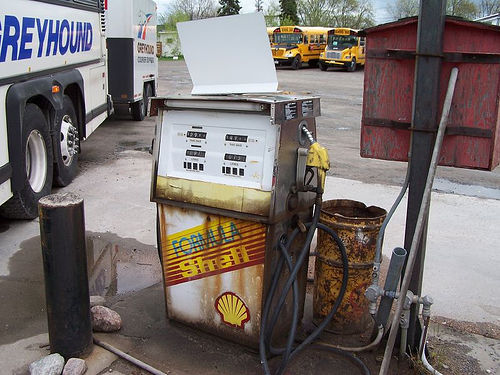
\includegraphics[trim={28mm 8mm 28mm 8mm},clip, width=\sizeP\textwidth]{fig/eval/hihd/ILSVRC2012_val_00045353.JPEG}
&
\fig[\sizeS]{eval/hihd/ILSVRC2012_val_00045353JPEG_smap_opticam.png} 
&  
\fig[\sizeS]{eval/hihd/ILSVRC2012_val_00045353JPEG_smap_scorecam.png} &
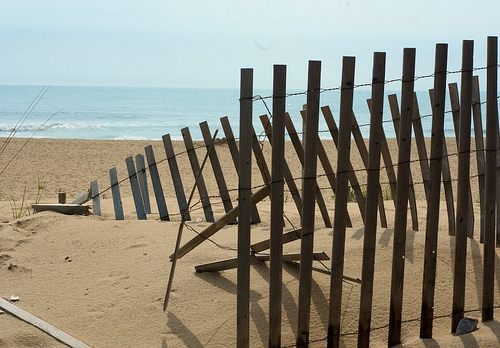
\includegraphics[trim={32mm 14mm 36mm 1mm},clip, width=\sizeP\textwidth]{fig/eval/hihd/ILSVRC2012_val_00041066.JPEG}
&
\fig[\sizeS]{eval/hihd/ILSVRC2012_val_00041066JPEG_smap_opticam.png} 
&          
\fig[\sizeS]{eval/hihd/ILSVRC2012_val_00041066JPEG_smap_scorecam.png} \\
gas pump&I$\uparrow$:66.3, D$\downarrow$:19.4&I$\uparrow$:94.2, D$\downarrow$:9.4&
worm fence&I$\uparrow$:69.7, D$\downarrow$:16.8&I$\uparrow$:91.9, D$\downarrow$:4.4\\
&AG$\uparrow$:100.0, AD$\downarrow$:0.0&AG$\uparrow$:0.0, AD$\downarrow$:0.0&
&AG$\uparrow$:73.2, AD$\downarrow$:0.0&AG$\uparrow$:0.0, AD$\downarrow$:28.8\\
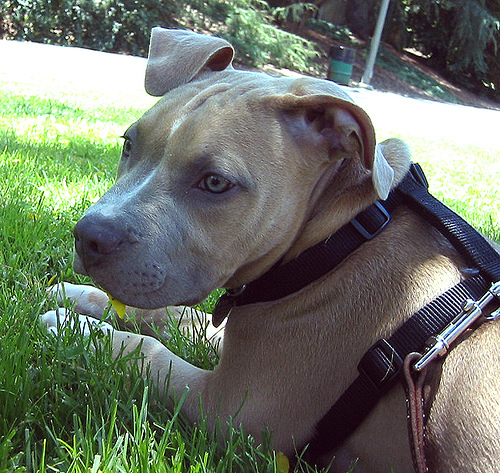
\includegraphics[trim={10mm 14mm 10mm 4mm},clip, width=\sizeP\textwidth]{fig/eval/hihd/ILSVRC2012_val_00040673.JPEG}
&        
\fig[\sizeS]{eval/hihd/ILSVRC2012_val_00040673JPEG_smap_opticam.png} 
&
\fig[\sizeS]{eval/hihd/ILSVRC2012_val_00040673JPEG_smap_scorecam.png} &
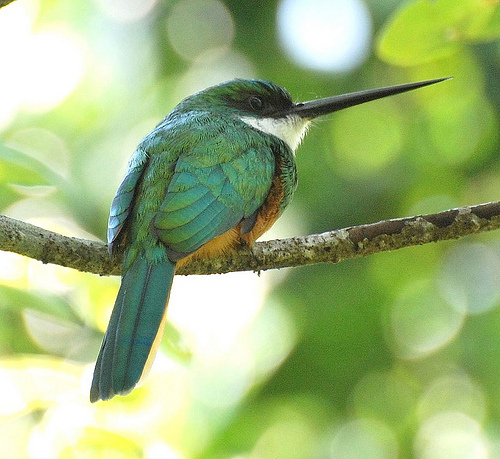
\includegraphics[trim={18mm 6mm 10mm 12mm},clip, width=\sizeP\textwidth]{fig/eval/hihd/ILSVRC2012_val_00030507.JPEG}
&
\fig[\sizeS]{eval/hihd/ILSVRC2012_val_00030507JPEG_smap_opticam.png} 
&                
\fig[\sizeS]{eval/hihd/ILSVRC2012_val_00030507JPEG_smap_scorecam.png} \\
staffordshire terrier&I$\uparrow$:62.1, D$\downarrow$:32.2&I$\uparrow$:93.4, D$\downarrow$:8.2&
jacamar&I$\uparrow$:66.3, D$\downarrow$:17.3&I$\uparrow$:94.6, D$\downarrow$:9.9\\
&AG$\uparrow$:41.3, AD$\downarrow$:0.0&AG$\uparrow$:0.0, AD$\downarrow$:0.3&
&AG$\uparrow$:91.4, AD$\downarrow$:0.0&AG$\uparrow$:56.5, AD$\downarrow$:0.0\\
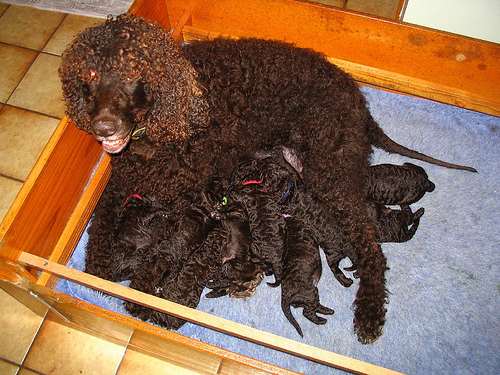
\includegraphics[trim={6mm 1mm 6mm 1mm},clip, width=\sizeP\textwidth]{fig/eval/hihd/ILSVRC2012_val_00029237.JPEG}
&
\fig[\sizeS]{eval/hihd/ILSVRC2012_val_00029237JPEG_smap_opticam.png} 
&     
\fig[\sizeS]{eval/hihd/ILSVRC2012_val_00029237JPEG_smap_scorecam.png} &
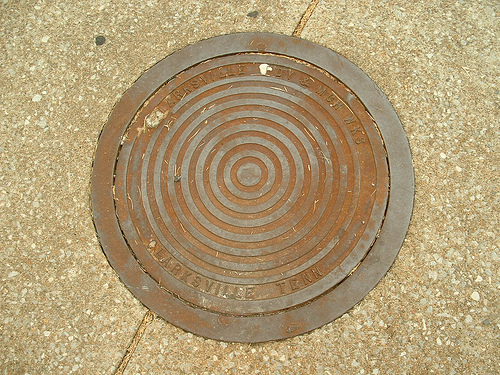
\includegraphics[trim={28mm 5mm 22mm 5mm},clip, width=\sizeP\textwidth]{fig/eval/hihd/ILSVRC2012_val_00005077.JPEG}
&
\fig[\sizeS]{eval/hihd/ILSVRC2012_val_00005077JPEG_smap_opticam.png} 
&          
\fig[\sizeS]{eval/hihd/ILSVRC2012_val_00005077JPEG_smap_scorecam.png} \\
Irish water spaniel&I$\uparrow$:52.6, D$\downarrow$:18.8&I$\uparrow$:90.5, D$\downarrow$:8.6&
manhole cover&I$\uparrow$:65.8, D$\downarrow$:29.6&I$\uparrow$92.7, D$\downarrow$:9.1\\
&AG$\uparrow$:86.4, AD$\downarrow$:0.0&AG$\uparrow$:65.1, AD$\downarrow$:0.0&
&AG$\uparrow$:24.0, AD$\downarrow$:0.0&AG$\uparrow$:0.0, AD$\downarrow$:59.9\\
% 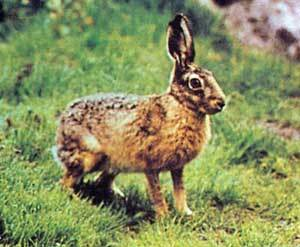
\includegraphics[trim={12mm 5mm 12mm 5mm},clip, width=\sizeP\textwidth]{fig/eval/hihd/ILSVRC2012_val_00003602.JPEG}
% &              
% \fig[\sizeS]{eval/hihd/ILSVRC2012_val_00003602JPEG_smap_opticam.png} 
% & 
% \fig[\sizeS]{eval/hihd/ILSVRC2012_val_00003602JPEG_smap_scorecam.png} \\
% hare&I$\uparrow$:61.3, D$\downarrow$:21.2&I$\uparrow$91.3, D$\downarrow$:8.9\\
% &AG$\uparrow$:93.7, AD$\downarrow$:0.0&AG$\uparrow$:0.0, AD$\downarrow$:0.6\\
\end{tabular}
\caption{Failure examples of Opti-CAM regarding insertion/deletion.}
\label{fig:hihd}
\end{figure}
%------------------------------------------------------------------------------

%------------------------------------------------------------------------------

\modify{

\subsection{More metrics}
In this section, we show additional metrics including AOPC~\citep{samek2016evaluating}, Max-Sensitivity~\citep{yeh2019fidelity} and ADCC~\citep{poppi2021revisiting}.
%
% \subsubsection{Definitions}
%
% \paragraph{AOPC.} Similar to \emph{Deletion}, AOPC considers removing the most relevant region first. After sorting the value of each position in saliency maps, instead of replacing them one by one with zero value, AOPC removes all pixels in a $9 \times 9$ neighborhood around the position by randomly sampled values from a uniform distribution. Then AOPC calculates the difference between the probability of the images $\vx$ and the probability of regions "deleted" from images $\vx$ and averages over the number of regions and over all images in the test set. Thus a larger value of AOPC implies the most sensitive regions are ranked first by saliency maps. 
%
% \paragraph{Max-Sensitvity (MS).} Given a network $f$, a function $S(\vx)$ to generate a saliency map for input images $\vx$ and a given input neighborhood radius $\epsilon$, then the max-sensitivity (MS) is define as
% \begin{equation}
%     MS \defn \max_{\|\vy-\vx\| \leq \epsilon} \| S(\vy) - S(\vx) \|.
% \end{equation}
%
% \paragraph{ADCC.} ADCC is a combination of three scores, \ie coherency (CH), complexity (CP), and Average Drop (AD). Let $S(\vx)$ denote the saliency maps for images $\vx$, $PCC(\vx,\vy)$ denote the function to calculate Pearson Correlation Coefficient between $\vx$ and $\vy$ and $\delta_{\vx}$ denote the standard deviation of $\vx$, the ADCC is define as
% \begin{align}
%     ADCC \defn & 3 ( \frac{1}{CH} + \frac{1}{1-CP} + \frac{1}{1-AD})^{-1}, \\
%     CH \defn & \frac{PCC(S(\vx),S(\vx \odot S(\vx)))}{\delta_{S(\vx)}\delta_{S(\vx \odot S(\vx))}},\\
%     CP \defn & \| S(\vx)\|_1.
% \end{align}
%
% \subsubsection{Resluts}
%
We use the code and suggested parameters of package Quantus\footnote{\url{https://github.com/understandable-machine-intelligence-lab/Quantus}} to measure AOPC and MS. In particular, patch size $14$ and number of evaluation regions $10$ for AOPC; lower bound $0.2$ and number of samples $10$ for MS.
For ADCC, we use the official code\footnote{\url{https://github.com/aimagelab/ADCC?fbclid=IwAR0YK_93lxp4pZQnt34SlA9aeNCLRX8m0u8yTZPxbTXi80qiyhTiqxWaQ7o}}.
We evaluate these metrics on ImageNet validation set using ResNet50 and VGG16. The results are reported in \autoref{tab:more-metrics-asked}. Since AOPC shares the same philosophy as I/D, it is not a surprise that Opti-CAM has poor performance on AOPC. Opti-CAM achieves the best performance on MS.
}

\begin{table}[]
\centering
\footnotesize
\setlength{\tabcolsep}{4pt}
\begin{tabular}{lrrr rrr} \toprule
\mr{2}{\Th{Method}} & \mc{3}{\Th{ResNet50}} & \mc{3}{\Th{VGG16}}  \\ \cmidrule{2-7}
                    & {{$AOPC\uparrow$}} & {{$MS\downarrow$}}& {{$ADCC\downarrow$}} & {{$AOPC\uparrow$}} & {{$MS\downarrow$}}& {{$ADCC\downarrow$}}  \\ \midrule
Grad-CAM~\citep{selvaraju2017grad}         &11.7&1.05&74.3&13.1&1.10&73.7        \\
Grad-CAM++~\cite{chattopadhay2018grad}     &11.6&1.04&73.6&11.6&1.09&74.6          \\
Score-CAM~\citep{wang2020score}            &10.2&1.04&61.0&11.0&1.09&73.9             \\
XGrad-CAM~\citep{fu2020axiom}              &11.9&1.05&74.3&13.1&1.10&73.9           \\
Ablation-CAM~\citep{ramaswamy2020ablation} &11.1&1.04&71.5&12.5&1.10&75.5          \\
Layer-CAM~\citep{jiang2021layercam} &\tb{13.0}&1.22&61.1&\tb{13.3}&1.25&51.7 \\
ExPerturbation~\citep{fong2019understanding}  &12.0&1.07&\tb{26.0}&11.2&1.09&\tb{42.8}  \\
\rowcolor{cyan!10}
Opti-CAM (ours)                            &6.3&\tb{1.03}&65.5&8.9&\tb{1.06}&70.0        \\ \bottomrule

    \end{tabular}
    \caption{\modify{\emph{AOPC/MS/ADCC} scores on ImageNet validation set; $\downarrow$ / $\uparrow$: lower / higher is better.}}
    \label{tab:more-metrics-asked}
\end{table}

% \begin{table}[]
% \centering
% \footnotesize
% \setlength{\tabcolsep}{4pt}
% \begin{tabular}{lrrr rrr rrr rrr} \toprule
% \mr{2}{\Th{Method}} & \mc{3}{\Th{ResNet50}} & \mc{3}{\Th{VGG16}} & \mc{3}{\Th{ViT-B}}& \mc{3}{\Th{DeiT-B}} \\ \cmidrule{2-13}
%                     & {{$AOPC\uparrow$}} & {{$MS\downarrow$}}& {{$ADCC\downarrow$}} & {{$AOPC\uparrow$}} & {{$MS\downarrow$}}& {{$ADCC\downarrow$}} & {{$AOPC\uparrow$}} & {{$MS\downarrow$}}& {{$ADCC\downarrow$}}& {{$AOPC\uparrow$}} & {{$MS\downarrow$}}& {{$ADCC\downarrow$}} \\ \midrule
% Grad-CAM~\citep{selvaraju2017grad}         &13.0&1.05&75.8&13.1&1.11&73.7     &&1.49&&&&       \\
% Grad-CAM++~\cite{chattopadhay2018grad}     &9.2&1.04&74.4&11.6&1.09&74.6     &&1.70&&&&       \\
% Score-CAM~\citep{wang2020score}            &11.3&1.04&&11.0&1.09&73.9     &&1.25&&&&          \\
% XGrad-CAM~\citep{fu2020axiom}              &13.2&1.05&&13.1&1.10&     &&1.49&&&&         \\
% Ablation-CAM~\citep{ramaswamy2020ablation} &12.4&1.04&&12.5&1.10&     &-&-&-&-&-&-        \\
% Layer-CAM~\citep{jiang2021layercam} &16.6&1.22&&13.3&1.25& &-&-&-&-&-&-\\
% ExPerturbation~\citep{fong2019understanding}  &14.5&1.07&&11.2&1.09&  &-&-&-&-&-&-\\
% RawAtt~\citep{dosovitskiy2020image}  &-&-&-&-&-&-   &&1.89&&&&\\
% Rollout~\citep{abnar2020quantifying} &-&-&-&-&-&-   &&1.27&&&&\\
% TIBAV~\cite{chefer2021transformer}&-&-&-&-&-&-   &&1.60&&&&\\
% \rowcolor{cyan!10}
% Opti-CAM (ours)                            &6.6&1.03&&8.9&1.06&         &&1.09&&&&\\ \bottomrule

%     \end{tabular}
%     \caption{Caption}
%     \label{tab:more-metrics-asked}
% \end{table}





%------------------------------------------------------------------------------

\section{Localization metrics}
\label{sec:loc-metrics}

Several works measure the localization ability of saliency maps, using metrics from the \emph{weakly-supervised object localization} (WSOL) task. While we show in the main paper that localization of the object and classifier interpretability are not well aligned as tasks, we still provide localization results here. We use the \emph{official metric} (OM), \emph{localization error} (LE), \emph{pixel-wise $F_1$ score}, \emph{box accuracy} (BoxAcc)~\citep{choe2020evaluating}, standard pointing game (SP)~\cite{zhang2018top}, \emph{energy pointing game} (EP)~\citep{wang2020score} and \emph{saliency metric} (SM)~\citep{dabkowski2017real} on the ILSVRC2014\footnote{\url{https://www.image-net.org/challenges/LSVRC/2014/index\#}} dataset. The goal of these metrics is to compare the saliency maps with bounding boxes around the object of interest. For simplicity, we define these metrics for a single image; the reported results are averaged over all images of the test set.

\subsection{Definitions}

We are given the saliency map $S^c$ obtained from test image $\vx$ for ground truth class $c$. We denote by $S^c_{\vp}$ its value at pixel $\vp$. We binarize the saliency map by thresholding at its average value and we take the bounding box of the largest connected component of the resulting mask as the predicted bounding box $B_p$, represented as a set of pixels. We compare this box against the set of ground truth bounding boxes $\cB$, which typically contains 1 or 2 boxes of the same class $c$, or with their union $U = \cup \cB$, again represented as a set of pixels. We also compare the predicted class label $c_p$ with the ground truth label $c$. All metrics take values in $[0,1]$ and are expressed as percentages, except SM~\eq{sm}, which is unbounded.

\paragraph{Official Metric (OM)}

measures the maximum overlap of the predicted bounding box with any ground truth bounding box, requiring that the predicted class label is correct:
\begin{equation}
	\OM \defn 1 - \paren{\max_{B \in \cB} \iou(B, B_p)} \ind_{c_p = c},
\label{eq:om}
\end{equation}
where $\iou$ is intersection over union.
% is defined as $\iou(B, B_p) \defn \frac{B \cap B_p}{B \cup B_p}$.

\paragraph{Localization Error (LE)}

is similar but ignores the predicted class label:
\begin{equation}
	\LE \defn 1 - \max_{B \in \cB} \iou(B, B_p).
\label{eq:le}
\end{equation}

\paragraph{Pixel-wise $F_1$ score (F1)}

is defined as $F_1 = 2 \frac{P R}{P + R}$, where \emph{precision} $P$ is the fraction of mass of the saliency map that is within the ground truth union
\begin{equation}
	P \defn \frac{\sum_{\vp \in U} S^c_{\vp}}{\sum_{\vp} S^c_{\vp}}
\label{eq:prec}
\end{equation}
and \emph{recall} $R$ is the fraction of the ground truth union that is covered by the saliency map
\begin{equation}
	R \defn \frac{\sum_{\vp \in U} S^c_{\vp}}{\card{U}}.
\label{eq:rec}
\end{equation}

\paragraph{Box Accuracy (BA)~\citep{choe2020evaluating}}

Given threshold values $\eta$ and $\delta$, we find the bounding box $B^\eta_p$ of the largest connected component of the binary mask $\set{\vp: S_{\vp} > \eta}$ and require that it overlaps by $\delta$ with at least one ground truth box:
\begin{equation}
	\BA(\eta, \delta) \defn \max_{B \in \cB} \ind_{\iou(B^\eta_p, B) \ge \delta}.
\label{eq:ba}
\end{equation}
After averaging over the test images, we take the maximum of this measure over a set of values $\eta$ and then the average over a set of values $\delta$.

\paragraph{Standard Pointing game (SP)~\cite{zhang2018top}}

We find the pixel $\vp^* \defn \arg\max_{\vp} S^c_{\vp}$ having the maximum saliency value and require that it lands in any of the ground truth bounding boxes:
\begin{equation}
	\spg \defn \ind_{\vp^* \in U}.
\label{eq:spg}
\end{equation}

\paragraph{Energy Pointing game (EP)~\citep{wang2020score}}

is equivalent to precision~\eq{prec}.

\paragraph{Saliency Metric (SM)~\citep{dabkowski2017real}}

penalizes the size of the predicted bounding box $B_p$ relative to the image and the cross-entropy loss:
\begin{equation}
	\SM \defn \log \max\paren{ 0.05, \frac{\card{B_p}}{hw} } - \log p^c,
\label{eq:sm}
\end{equation}
where $h \times w$ is the input image resolution and $p^c$ is the precicted probability for ground truth class label $c$.

%------------------------------------------------------------------------------
\begin{table}[ht]
\centering
\footnotesize
\setlength{\tabcolsep}{4pt}
\renewcommand{\arraystretch}{0.8}
\begin{tabular}{lccc|cccc|ccc|cccc} \toprule
\mr{2}{\Th{method}} 
&\mc{7}{\Th{ResNet50}} &\mc{7}{\Th{VGG16}}    \\ \cmidrule{2-15}
& {OM$\downarrow$} & {LE$\downarrow$} & {F1$\uparrow$}&{BA$\uparrow$}& {SP$\uparrow$} & {EP$\uparrow$} & {SM$\downarrow$} & {OM$\downarrow$} & {LE$\downarrow$} & {F1$\uparrow$}&{BA$\uparrow$}& {SP$\uparrow$} & {EP$\uparrow$} & {SM$\downarrow$} \\ \midrule

Fake-CAM~\citep{poppi2021revisiting}               &63.6&54.0&57.7&47.9&99.8&28.5&0.98
&64.7&54.0&57.7&47.9&99.8&28.5&1.07\\ \midrule
Grad-CAM~\citep{selvaraju2017grad}         &72.9&65.8&49.8&\tb{56.2}&69.8&33.3&1.30 
&71.1&62.3&42.0&54.2&64.8&32.0&1.39\\
Grad-CAM++~\cite{chattopadhay2018grad}     &73.1&66.1&\tb{50.4}&\tb{56.2}&69.9&33.1&1.29   
&70.8&61.9&44.3&55.2&66.2&32.3&1.38  \\
Score-CAM~\citep{wang2020score}            &\tb{72.2}&64.9&49.6&54.5&68.7&32.4&\tb{1.25}   
&71.2&62.5&\tb{45.3}&\tb{58.5}&\tb{68.2}&33.4&1.40 \\
Ablation-CAM~\citep{ramaswamy2020ablation} &72.8&65.7&50.2&56.1&69.9&33.1&1.26      
&71.3&62.6&43.2&56.2&65.7&32.7&1.39 \\
XGrad-CAM~\citep{fu2020axiom}              &72.9&65.8&49.8&\tb{56.2}&69.8&33.3&1.30  
&70.8&62.0&41.9&53.5&64.4&31.6&1.41 \\
Layer-CAM~\citep{jiang2021layercam} &73.1&66.0&50.1&55.5&\tb{70.0}&33.0&1.29
&70.5&61.5&28.0&54.7&65.0&32.4&1.45\\
ExPerturbation~\citep{fong2019understanding}  &73.6&66.6&37.5&44.2&64.8&\tb{38.2}&1.59
&74.1&66.4&37.8&43.3&62.7&\tb{36.1}&1.74\\
\rowcolor{cyan!10}
Opti-CAM (ours)                            &\tb{72.2}&\tb{64.8}&47.3&49.2&59.4&30.5&1.34         
&\tb{69.1}&\tb{59.9}&44.1&51.2&61.4&30.7&\tb{1.34}   \\ 
% \midrule
% \mc{8}{\Th{VGG16}}                        \\ \midrule
% Fake-CAM~\citep{poppi2021revisiting}               &64.7&54.0&57.7&47.9&99.8&28.5&1.07 \\ \midrule
% Grad-CAM~\citep{selvaraju2017grad}         &71.1&62.3&42.0&54.2&64.8&32.0&1.39            \\
% Grad-CAM++~\cite{chattopadhay2018grad}     &70.8&61.9&44.3&55.2&66.2&32.3&1.38           \\
% Score-CAM~\citep{wang2020score}            &71.2&62.5&\tb{45.3}&\tb{58.5}&\tb{68.2}&33.4&1.40             \\
% Ablation-CAM~\citep{ramaswamy2020ablation} &71.3&62.6&43.2&56.2&65.7&32.7&1.39            \\
% XGrad-CAM~\citep{fu2020axiom}              &70.8&62.0&41.9&53.5&64.4&31.6&1.41             \\
% Layer-CAM~\citep{jiang2021layercam} &70.5&61.5&28.0&54.7&65.0&32.4&1.45\\
% ExPerturbation~\citep{fong2019understanding}  &74.1&66.4&37.8&43.3&62.7&\tb{36.1}&1.74\\
% \rowcolor{cyan!10}
% Opti-CAM (ours)                            &\tb{69.1}&\tb{59.9}&44.1&51.2&61.4&30.7&\tb{1.34}        \\ 
\bottomrule
\end{tabular}
% \vspace{6pt}
\caption{\emph{Localization metrics} on ImageNet validation set. OM: \emph{official metric}; LE: \emph{localization error}; F1: \emph{pixel-wise $F_1$ score}; BA: box accuracy; SP: standard pointing game; EP: energy pointing game; SM: \emph{saliency metric}. $\downarrow$ / $\uparrow$: lower / higher is better. Bold: best, excluding Fake-CAM.}
\label{tab:imagenet-loc}
% \vspace{-0.4cm}
\end{table}
%------------------------------------------------------------------------------
%------------------------------------------------------------------------------
\begin{table}[t]
\centering
\footnotesize
%\setlength{\tabcolsep}{3pt}
\setlength{\tabcolsep}{4pt}
\begin{tabular}{lrrr|rrrr|rrr|rrrr}
\toprule
\mr{2}{\Th{method}} &\mc{7}{ViT-B}&\mc{7}{DeiT-B}\\ \cmidrule{2-15}
& {OM$\downarrow$} & {LE$\downarrow$} & {F1$\uparrow$}&{BA$\uparrow$}& {SP$\uparrow$} & {EP$\uparrow$} & {SM$\downarrow$}  & {OM$\downarrow$} & {LE$\downarrow$} & {F1$\uparrow$}&{BA$\uparrow$}& {SP$\uparrow$} & {EP$\uparrow$} & {SM$\downarrow$} \\ \midrule

Fake-CAM~\citep{poppi2021revisiting}   &62.8&54.0&57.7&47.9&99.8&28.6&0.87 
&61.4&54.0&57.7&47.9&99.8&28.7&0.83\\ \midrule
Grad-CAM~\citep{selvaraju2017grad}                   &79.6&74.3&29.4&45.0&58.1&31.0&3.27
&65.5&60.3&44.3&47.2&{62.8}&{30.2}&1.20\\
Grad-CAM++~\cite{chattopadhay2018grad}               &84.2&80.6&14.8&23.8&51.4&27.3&4.15
&70.6&67.2&34.3&43.6&57.7&30.3&2.14\\
Score-CAM~\citep{wang2020score}                   &77.6&71.6&46.0&54.3&\tb{66.1}&33.1&3.14 
&79.9&76.2&31.9&43.8&\tb{63.4}&32.2&3.14\\
%Ablation-CAM~\citep{ramaswamy2020ablation}     &&&&       &&&&&&&\\
XGrad-CAM~\citep{fu2020axiom}                      &82.0&76.9&19.6&41.3&52.8&28.5&3.31
&82.0&78.4&19.5&44.1&53.4&28.8&3.03\\
Layer-CAM~\citep{jiang2021layercam}&70.7&63.9&20.6&50.5&60.7&32.6&1.44
&80.2&77.3&17.6&50.8&62.7&35.1&3.15\\
ExPerturbation~\citep{fong2019understanding}&71.5&64.9&35.9&44.6&62.3&\tb{35.3}&1.34
&69.9&64.3&36.2&44.2&63.1&\tb{35.5}&1.16\\
RawAtt~\citep{dosovitskiy2020image}  &72.4&64.8&18.5&50.4&55.4&31.6&1.68
&73.5&68.2&5.9&\tb{48.1}&46.5&27.3&1.91\\
Rollout~\citep{abnar2020quantifying} &67.6&58.8&36.9&50.7&57.8&30.0&1.16
&63.9&57.0&27.8&47.9&36.5&27.2&0.94\\
TIBAV~\cite{chefer2021transformer}&70.1&63.1&26.6&\tb{58.8}&\tb{66.1}&35.0&1.23
&68.2&62.2&28.1&59.6&64.1&33.5&1.08\\
\rowcolor{cyan!10}
Opti-CAM (ours)     
&\tb{64.4}&\tb{54.6}&\tb{54.5}&48.0&58.2&28.7&\tb{0.98}
&\tb{62.3}&\tb{55.1}&\tb{53.9}&48.0&55.1&28.8&\tb{0.84}\\
% \midrule
%  \mc{8}{DeiT-B} \\ \midrule
% Fake-CAM~\citep{poppi2021revisiting}    &61.4&54.0&57.7&47.9&99.8&28.7&0.83 \\ \midrule
% Grad-CAM~\citep{selvaraju2017grad}                 &65.5&60.3&44.3&47.2&{62.8}&{30.2}&1.20\\
% Grad-CAM++~\cite{chattopadhay2018grad}             &70.6&67.2&34.3&43.6&57.7&30.3&2.14\\
% Score-CAM~\citep{wang2020score}                  &79.9&76.2&31.9&43.8&\tb{63.4}&32.2&3.14 \\
% %Ablation-CAM~\citep{ramaswamy2020ablation}     &&&&       &&&&&&&\\
% XGrad-CAM~\citep{fu2020axiom}                      &82.0&78.4&19.5&44.1&53.4&28.8&3.03\\
% Layer-CAM~\citep{jiang2021layercam}&80.2&77.3&17.6&50.8&62.7&35.1&3.15\\
% ExPerturbation~\citep{fong2019understanding}&69.9&64.3&36.2&44.2&63.1&\tb{35.5}&1.16\\
% RawAtt~\citep{dosovitskiy2020image} &73.5&68.2&5.9&\tb{48.1}&46.5&27.3&1.91\\
% Rollout~\citep{abnar2020quantifying} &63.9&57.0&27.8&47.9&36.5&27.2&0.94\\
% TIBAV~\cite{chefer2021transformer}&68.2&62.2&28.1&59.6&64.1&33.5&1.08\\
% \rowcolor{cyan!10}
% Opti-CAM     
% &\tb{62.3}&\tb{55.1}&\tb{53.9}&48.0&55.1&28.8&\tb{0.84}\\
\bottomrule
\end{tabular}
\vspace{5pt}
\caption{\emph{Localization metrics} with ViT and DeiT on ImageNet validation set. OM: \emph{official metric}; LE: \emph{localization error}; F1: \emph{pixel-wise $F_1$ score}; BA: box accuracy;
SP: standard pointing game; EP: energy pointing game; SM: \emph{saliency metric}.
$\downarrow$ / $\uparrow$: lower / higher is better. Bold: best, excluding Fake-CAM.}
\label{tab:ablate-loc-sup-deit}
\end{table}
%%%%%%%%%%%%%%%%%%%%%%%%%%%%%%%%%%
%------------------------------------------------------------------------------

\subsection{Results}

We evaluate the localization ability of saliency maps obtained by our Opti-CAM and we compare with other attribution methods quantitatively. \autoref{tab:imagenet-loc} and \autoref{tab:ablate-loc-sup-deit} report localization metrics on ImageNet. We observe different behavior in different metrics. In particular, Opti-CAM on ResNet and VGG performs best on OM and LE but poorly on the remaining metrics. On transformers, Opti-CAM performs best on OM, LE, F1, and SM.

Metrics, where Opti-CAM does not perform well, are mostly the ones that penalize saliency maps that are more spread out. For example, SP and EP penalize saliency outside the ground truth bounding box of an object. This is not necessarily a weakness of Opti-CAM, because rather than weakly supervised object localization, the objective here is to explain how the classifier works.

%------------------------------------------------------------------------------


\section{Medical data}
\label{sec:medical}

Medical image recognition is a high-stakes task that crucially needs interpretable models. We thus evaluate our method on two standard medical image classification datasets.

\subsection{Datasets}

\paragraph{Chest X-ray}

\citep{kermany2018labeled} aims at recognizing chest images of patients with pneumonia from healthy ones with $5,216$ training images, $16$ for validation and $624$ for testing. Images are resized to $224 \times 224 \times 3$ to adapt to the pretrained models.

\paragraph{Kvasir}

\citep{pogorelov2017kvasir} contains $8$ classes and aims at recognizing anatomical landmarks, pathological findings and endoscopic procedures inside the gastrointestinal tract. The $8,000$ images are split into $6,000$ images for training, $1,000$ for validation and $1,000$ for testing. Images are resized as for the other datasets

\subsection{Network fine-tuning}

To train our models on the medical data, we first train the last fully-connected layer according to the classes in each dataset, while keeping the backbone frozen. On Chest X-ray, we use learning rate  $10^{-3}$ for both networks. On Kvasir, we use learning rate $10^{-4}$ for ResNet50 and $5\times10^{-3}$ for VGG16. We then fine-tune the entire network with a learning rate $10^{-5}$ for 50 epochs, using SGD with momentum 0.9 for both networks on both datasets. On Chest X-ray data, we obtain accuracies of $83.2\%$ for VGG16 and $82.0\%$ for ResNet50; on Kvasir, $89.5\%$ for VGG16 and $89.8\%$ for ResNet50.

%------------------------------------------------------------------------------
\begin{table}
\centering
\footnotesize
\setlength{\tabcolsep}{4pt}
\renewcommand{\arraystretch}{0.8}
\begin{tabular}{lrrr|rrr|rrr|rrr} \toprule

 \mr{3}{\Th{Method}}                  
&\mc{6}{\Th{Chest X-ray}}   & \mc{6}{\Th{Kvasir}}  \\ \cmidrule{2-13}
 & \mc{3}{\Th{ResNet50}}                                                  & \mc{3}{\Th{VGG16}}& \mc{3}{\Th{ResNet50}}                                                  & \mc{3}{\Th{VGG16}} \\
\cmidrule{2-13}
                               & {$\AD\!\downarrow$} & {$\AG\!\uparrow$} & {$\AI\!\uparrow$} & {$\AD\!\downarrow$} & {$\AG\!\uparrow$} & {$\AI\!\uparrow$} & {$\AD\!\downarrow$} & {$\AG\!\uparrow$} & {$\AI\!\uparrow$} & {$\AD\!\downarrow$} & {$\AG\!\uparrow$} & {$\AI\!\uparrow$}\\ \midrule

 Fake-CAM~\citep{poppi2021revisiting} &0.1&0.9&49.7&0.1&0.4&29.8 &0.1&0.4&48.3&0.0&0.3&45.0\\\midrule
 Grad-CAM~\citep{selvaraju2017grad}         &20.4&29.7&48.7&36.8&39.8&42.3  &10.0&23.2&39.8&33.8&6.3&14.6\\
 Grad-CAM++~\cite{chattopadhay2018grad}     &24.7&24.1&41.2&36.9&43.4&45.8  &11.2&18.7&32.9&20.7&9.3&20.4\\
 Score-CAM~\citep{wang2020score}            &21.6&27.7&44.2&35.3&47.4&48.9  &9.1&26.7&40.8&8.4&24.0&39.4\\
 Ablation-CAM~\citep{ramaswamy2020ablation} &26.2&27.9&42.9&36.9&46.9&47.8  &10.7&21.6&35.4&10.6&20.9&36.9\\
 XGrad-CAM~\citep{fu2020axiom}              &20.4&29.7&48.7&34.7&47.3&50.2  &10.0&23.2&39.8&12.1&21.6&35.2\\
 Layer-CAM~\citep{jiang2021layercam} &24.5&23.4&39.1&36.6&45.9&47.6  &11.7&18.2&32.5&12.9&17.1&30.8\\
 ExPerturbation~\citep{fong2019understanding}&21.4&5.5&17.9&29.7&21.8&28.7  &48.4&13.8&21.0&34.8&19.0&27.7\\
 \rowcolor{cyan!10}
 Opti-CAM (ours)                            &\tb{0.1}&\tb{91.2}&\tb{98.4}&\tb{0.0}&\tb{85.9}&\tb{86.2}  &\tb{0.2}&\tb{91.1}&\tb{99.0}&\tb{0.0}&\tb{93.5}&\tb{98.1}\\
% \midrule
% \mc{7}{\Th{Kvasir}}     \\ \midrule
%  Fake-CAM~\citep{poppi2021revisiting} &0.1&0.4&48.3&0.0&0.3&45.0\\\midrule
%  Grad-CAM~\citep{selvaraju2017grad}         &10.0&23.2&39.8&33.8&6.3&14.6\\
%  Grad-CAM++~\cite{chattopadhay2018grad}     &11.2&18.7&32.9&20.7&9.3&20.4\\
% Score-CAM~\citep{wang2020score}            &9.1&26.7&40.8&8.4&24.0&39.4\\
%  Ablation-CAM~\citep{ramaswamy2020ablation} &10.7&21.6&35.4&10.6&20.9&36.9\\
%  XGrad-CAM~\citep{fu2020axiom}              &10.0&23.2&39.8&12.1&21.6&35.2\\
%  Layer-CAM~\citep{jiang2021layercam} &11.7&18.2&32.5&12.9&17.1&30.8\\
%  ExPerturbation~\citep{fong2019understanding}&48.4&13.8&21.0&34.8&19.0&27.7\\
%  \rowcolor{cyan!10}
%  Opti-CAM (ours)                            &\tb{0.2}&\tb{91.1}&\tb{99.0}&\tb{0.0}&\tb{93.5}&\tb{98.1}\\
 \bottomrule
\end{tabular}
% \vspace{6pt}
\caption{\emph{Classification metrics} on Chest X-ray and KVASIR datasets. $\AD$/$\AI$: average drop/increase~\citep{chattopadhay2018grad}; $\AG$: average gain (ours); $\downarrow$ / $\uparrow$: lower / higher is better; Bold: best, excluding Fake-CAM.}
\label{tab:xray-n-kvasir}
\end{table}
%------------------------------------------------------------------------------


%------------------------------------------------------------------------------
\begin{table}[ht!]
%\vspace{-0.2cm}
\centering
\footnotesize
\setlength{\tabcolsep}{4pt}
\begin{tabular}{lrr rr rr rr} \toprule

 \mr{3}{\Th{Method}}                  
&\mc{4}{\Th{Chest X-ray}}   & \mc{4}{\Th{Kvasir}}  \\ \cmidrule{2-9}
 & \mc{2}{\Th{ResNet50}}                                                  & \mc{2}{\Th{VGG16}}& \mc{2}{\Th{ResNet50}}                                                  & \mc{2}{\Th{VGG16}} \\
\cmidrule{2-9}
                             & {{I$\uparrow$}} & {{D$\downarrow$}} & {{I$\uparrow$}} & {{D$\downarrow$}} & {{I$\uparrow$}} & {{D$\downarrow$}}  & {{I$\uparrow$}} & {{D$\downarrow$}} \\ \midrule
  Grad-CAM~\citep{selvaraju2017grad}         &83.0&75.7&85.0&81.9&\tb{81.3}&\tb{32.2}&72.1&48.9\\
  Grad-CAM++~\cite{chattopadhay2018grad}     &82.2&79.1&85.1&81.8&80.2&33.8&72.1&48.7\\
  Score-CAM~\citep{wang2020score}            &82.9&77.0&87.6&79.0&80.6&33.4&79.3&34.9\\
  Ablation-CAM~\citep{ramaswamy2020ablation} &\tb{83.5}&\tb{75.1}&\tb{92.0}&\tb{73.1}&80.3&32.6&\tb{79.4}&36.2\\
  XGrad-CAM~\citep{fu2020axiom}              &82.9&75.6&88.7&75.6&\tb{81.3}&\tb{32.2}&79.2&36.6\\
  Opti-CAM (ours)                            &82.0&78.4&86.8&79.5&80.2&37.7&77.0&\tb{24.8}\\

 \bottomrule
\end{tabular}
\vspace{3pt}
\caption{\modify{I/D: insertion/deletion~\citep{petsiuk2018rise} on Chest X-ray and KVASIR dataset using both \Th{ResNet50} and \Th{VGG16}. $\downarrow$ / $\uparrow$: lower / higher is better.}}
\label{tab:xray-n-kvasir-ID}
\vspace{-0.4cm}
\end{table}
%------------------------------------------------------------------------------


\subsection{Results}

\autoref{tab:xray-n-kvasir} reports metrics \modify{AD/AG/AI and \autoref{tab:xray-n-kvasir-ID} reports metrics I/D} on Chest X-ray and Kvasir using \Th{ResNet50} and \Th{VGG16} networks. The conclusions remain the same as for ImageNet. \modify{Opti-CAM achieves an average performance on I/D and performs best D on VGG16 of KVASIR.} More than that, AD and AI are near perfect in most cases and AG is also extremely high.
Additional visualizations are presented in supplementary material.
%Additional visualizations are presented in Section \autoref{sec:more-vis}.


%------------------------------------------------------------------------------

\section{More ablations}
\label{sec:more-ablation}

\subsection{Selectivity}

We investigate the effect of the selectivity of saliency maps on classification performance. In particular, before evaluation, we raise saliency maps element-wise to an exponent $\alpha$ that takes values in $\{0.01,0.05,0.1,0.5,1,1.5,2,3,5,10\}$. When $\alpha$ is small, the saliency maps become more uniform, so that more information about the original image is revealed to the network. Respectively, when $\alpha$ is large, the saliency maps become more selective, so that the network sees fewer parts of the input. The order of pixels is maintained.

%------------------------------------------------------------------------------
\begin{figure}[htp!]
\tiny
\centering
\setlength{\tabcolsep}{3pt}
\footnotesize
\begin{tabular}{ccc}
\centering
\extfig{AD}{
\begin{tikzpicture}
\begin{axis}[
	height=4.2cm,
	width=4.6cm,
	ylabel={AD$\downarrow$},
	xlabel={$\alpha$},
	legend pos=outer north east,
]
	\addplot[mark=*,blue] table{fig/eval/adaiag/maskin_AblationCAM_ad.txt}; \leg{Ablation-CAM}
	\addplot[mark=*,red] table{fig/eval/adaiag/maskin_GradCAM_ad.txt}; \leg{Grad-CAM}
	\addplot[mark=*,green] table{fig/eval/adaiag/maskin_GradCAMPlusPlus_ad.txt}; \leg{Grad-CAM++}
	\addplot[mark=*,black] table{fig/eval/adaiag/maskin_XGradCAM_ad.txt}; \leg{XGrad-CAM}
	\addplot[mark=*,brown] table{fig/eval/adaiag/maskin_ScoreCAM_ad.txt}; \leg{Score-CAM}
	\addplot[mark=*,orange] table{fig/eval/adaiag/maskin_versionP0_ad.txt}; \leg{Opti-CAM}
    \legend{};
\end{axis}
\end{tikzpicture}
}
&
\extfig{AG}{
\begin{tikzpicture}
\begin{axis}[
	height=4.2cm,
	width=4.6cm,
	ylabel={AG$\uparrow$},
	xlabel={$\alpha$},
	legend pos=outer north east,
]
	\addplot[mark=*,blue] table{fig/eval/adaiag/maskin_AblationCAM_ag.txt}; \leg{Ablation-CAM}
	\addplot[mark=*,red] table{fig/eval/adaiag/maskin_GradCAM_ag.txt}; \leg{Grad-CAM}
	\addplot[mark=*,green] table{fig/eval/adaiag/maskin_GradCAMPlusPlus_ag.txt}; \leg{Grad-CAM++}
	\addplot[mark=*,black] table{fig/eval/adaiag/maskin_XGradCAM_ag.txt}; \leg{XGrad-CAM}
	\addplot[mark=*,brown] table{fig/eval/adaiag/maskin_ScoreCAM_ag.txt}; \leg{Score-CAM}
	\addplot[mark=*,orange] table{fig/eval/adaiag/maskin_versionP0_ag.txt}; \leg{Opti-CAM}
	\legend{};
\end{axis}
\end{tikzpicture}
}
&

\extfig{AI}{
\begin{tikzpicture}
\begin{axis}[
	height=4.2cm,
	width=4.6cm,
	ylabel={AI$\uparrow$},
	xlabel={$\alpha$},
	legend pos=outer north east,
]
	\addplot[mark=*,blue] table{fig/eval/adaiag/maskin_AblationCAM_ai.txt}; \leg{Ablation-CAM}
	\addplot[mark=*,red] table{fig/eval/adaiag/maskin_GradCAM_ai.txt}; \leg{Grad-CAM}
	\addplot[mark=*,green] table{fig/eval/adaiag/maskin_GradCAMPlusPlus_ai.txt}; \leg{Grad-CAM++}
	\addplot[mark=*,black] table{fig/eval/adaiag/maskin_XGradCAM_ai.txt}; \leg{XGrad-CAM}
	\addplot[mark=*,brown] table{fig/eval/adaiag/maskin_ScoreCAM_ai.txt}; \leg{Score-CAM}
	\addplot[mark=*,orange] table{fig/eval/adaiag/maskin_versionP0_ai.txt}; \leg{Opti-CAM}
\end{axis}
\end{tikzpicture}
}\\

\end{tabular}
\caption{Effect of \emph{selectivity} (raising element-wise to exponent $\alpha$) of saliency maps on classification performance. $\AD$/$\AI$: average drop/increase~\citep{chattopadhay2018grad}; $\AG$: average gain (ours); $\downarrow$ / $\uparrow$: lower / higher is better.}
\label{fig:aiadag-alpha}
\end{figure}
%------------------------------------------------------------------------------

Results in terms of $\AD, \AG, \AI$ are shown in \autoref{fig:aiadag-alpha}, averaged over $1,000$ ImageNet images. We observe that $\AD$ stays near zero for Opti-CAM for $\alpha < 2$, while it increases linearly with $\alpha$ for the other methods. The $\AG$ and $\AI$ of Opti-CAM has a strong peak at $\alpha = 1$, \ie for the original saliency maps. The other methods are less sensitive and their $\AI$ performance is not optimal at $\alpha = 1$.

%------------------------------------------------------------------------------

\subsection{Opti-CAM components}

\paragraph{Objective function}

We consider more alternative definitions of the objective function $F^c_\ell$, taking into account not only the regions inside the saliency maps (In) but also their complement, outside (Out). In particular, relative to \Fdef, we define \MIODref as
\begin{equation}
	F^c_\ell(\vx; \vu) \defn g_c(f(\vx \odot \Vs)) - g_c(f(\vx \odot (1-\Vs))),
\label{eq:mi-dref}
\end{equation}
where $\Vs \defn n(\up(S_\ell(\vx; \vu)))$ for brevity. Similarly, relative to \Fref, we define \MIOFref as
\begin{equation}
\begin{split}
	F^c_\ell(\vx; \vu) \defn
		- \abs{g_c(f(\vx)) - g_c(f(\vx \odot \Vs))} \\
		+ \abs{g_c(f(\vx)) - g_c(f(\vx \odot (1-\Vs)))}.
\end{split}
\label{eq:mi-ref}
\end{equation}

According to \autoref{tab:ablate-loss}, \MIODref performs great on AD and AI but worse on AG, while \MIOFref is worse on all metrics. Therefore, including the complementary of the saliency map is not beneficial.

%------------------------------------------------------------------------------
\begin{table}[t]
\centering
%\small
\footnotesize
\setlength{\tabcolsep}{4pt}
\renewcommand{\arraystretch}{0.8}
\begin{tabular}{lcrrrrr} \toprule
{\Th{Method}} & {$F^c_\ell$}& {$\AD\!\downarrow$}& {$\AG\!\uparrow$} & {$\AI\!\uparrow$}  \\ \midrule
Fake-CAM~\citep{poppi2021revisiting}              &          &     0.5  &      0.7  &     42.1  \\ \midrule
Grad-CAM~\citep{selvaraju2017grad}                &          &    15.0  &     15.3  &     40.4  \\
Grad-CAM++~\cite{chattopadhay2018grad}            &          &    16.5  &     10.6  &     35.2  \\
Score-CAM~\citep{wang2020score}                   &          &    12.5  &     16.1  &     42.6  \\
Ablation-CAM~\citep{ramaswamy2020ablation}        &          &    15.1  &     13.5  &     39.9  \\
XGrad-CAM~\citep{fu2020axiom}                     &          &    14.3  &     15.1  &     42.1  \\
Layer-CAM~\citep{jiang2021layercam}               &          &    49.2  &      2.7  &     12.7  \\
ExPerturbation~\citep{fong2019understanding}      &          &    43.8  &      7.1  &     18.9  \\
\midrule
\mr{4}{Opti-CAM}
& \Fdef~\eq{obj}        &1.4          & \tb{66.3} &92.5\\
& \Fref~\eq{ref}        &7.1&18.5&54.9     \\
& \MIODref~\eq{mi-dref} &\tb{0.2}&5.5&\tb{99.7}\\
& \MIOFref~\eq{mi-ref}  &25.9&7.6&42.6\\
\bottomrule
\end{tabular}
% \vspace{3pt}
\caption{\emph{Ablation study on objective function} using VGG16 on 1000 images of ImageNet validation set.
Choices for objective function $F^c_\ell$: \Fdef:~\eq{obj}; \Fref:~\eq{ref}; \MIODref:~\eq{mi-dref}; \MIOFref:~\eq{mi-ref}.
Choice for normalization function $n$: Range~\eq{n-rng}. Iterations: 50.
$\AD$/$\AI$: average drop/increase~\citep{chattopadhay2018grad}; $\AG$: average gain (ours); $\downarrow$ / $\uparrow$: lower / higher is better.}
\label{tab:ablate-loss}
\end{table}
%------------------------------------------------------------------------------

%------------------------------------------------------------------------------
\begin{table}[ht!]
\footnotesize
\centering
\setlength{\tabcolsep}{6pt}
\renewcommand{\arraystretch}{0.8}
\begin{tabular}{crrr|crrr} \toprule
{\Th{Layer}} & {$\AD\!\downarrow$}& {$\AG\!\uparrow$} & {$\AI\!\uparrow$} & {\Th{Layer}} & {$\AD\!\downarrow$}& {$\AG\!\uparrow$} & {$\AI\!\uparrow$} \\ \midrule
42 &1.4&66.0&92.5&
36 &1.7&66.1&90.3\\
32 &2.8&61.3&81.6&
29 &1.6&78.0&93.9\\
26 &1.7&80.1&93.7&
22 &3.3&68.8&84.8\\
19 &2.9&67.3&84.9&
16 &2.3&72.4&89.1\\
12 &4.1&61.9&82.4&
9  &4.3&44.2&71.9\\
6  &13.5&23.5&50.2&&&&\\ \bottomrule
\end{tabular}
% \vspace{5pt}
\caption{\emph{Layer ablation} on $1,000$ images from ImageNet validation set, using various layers of VGG16. The last convolutional layer before max pooling is chosen as our default layer (layer 42). $\AD$/$\AI$: average drop/increase~\citep{chattopadhay2018grad}; $\AG$: average gain (ours); $\downarrow$ / $\uparrow$: lower / higher is better.}
\label{tab:layer}
\end{table}
%------------------------------------------------------------------------------

\paragraph{Layers}

\autoref{tab:layer} shows how the performance of Opti-CAM, in terms of AD/AI/AG, depends on the layer $\ell$ of the VGG16 network used to compute the saliency map $S^c_\ell$~\eq{v-sal}. We can see that the layers 26, 29, and 42 are all competitive. We choose the last convolutional layer (42) to be compatible with the other CAM methods \citep{zhou2016learning,selvaraju2017grad,chattopadhay2018grad,wang2020score}.

%------------------------------------------------------------------------------
\begin{figure}[hpt]
%\vspace{-0.2cm}
\centering
\begin{tabular}{ccc}
\extfig{ab-ad}{
\begin{tikzpicture}
\begin{axis}[
    yticklabel style={
            /pgf/number format/fixed,
            /pgf/number format/precision=5
    },
    scaled y ticks=false,
	height=4.2cm,
	width=4.6cm,
	xlabel={Iterations},
	ylabel={AD},
%	legend style={at={(1,1)},anchor=north east,font=\scriptsize},
]
	\addplot[mark=*,blue] table[x index=0, y index=1]{\plotAD};\leg{$\eta=0.01$}
	\addplot[mark=*,orange] table[x index=0, y index=2]{\plotAD};\leg{$\eta=0.03$}
	\addplot[mark=*,black] table[x index=0, y index=3]{\plotAD};\leg{$\eta=0.05$}
	\addplot[mark=*,olive] table[x index=0, y index=4]{\plotAD};\leg{$\eta=0.08$}
	\addplot[mark=*,green] table[x index=0, y index=5]{\plotAD};\leg{$\eta=0.1$}
 \legend{}
\end{axis}
\end{tikzpicture}
}&
\extfig{ab-ag}{
\begin{tikzpicture}
\begin{axis}[
    yticklabel style={
            /pgf/number format/fixed,
            /pgf/number format/precision=5
    },
    scaled y ticks=false,
	height=4.2cm,
	width=4.6cm,
	xlabel={Iterations},
	ylabel={AG},
%	legend style={at={(1,1)},anchor=north east,font=\scriptsize},
	legend pos=south east,
]
	\addplot[mark=*,blue] table[x index=0, y index=1]{\plotAG};\leg{$\eta=0.01$}
	\addplot[mark=*,orange] table[x index=0, y index=2]{\plotAG};\leg{$\eta=0.03$}
	\addplot[mark=*,black] table[x index=0, y index=3]{\plotAG};\leg{$\eta=0.05$}
	\addplot[mark=*,olive] table[x index=0, y index=4]{\plotAG};\leg{$\eta=0.08$}
	\addplot[mark=*,green] table[x index=0, y index=5]{\plotAG};\leg{$\eta=0.1$}
 \legend{}
\end{axis}
\end{tikzpicture}
}
&
\extfig{ab-ai}{
\begin{tikzpicture}
\begin{axis}[
	height=4.2cm,
	width=4.6cm,
	xlabel={Iterations},
	ylabel={AI},
%	legend style={at={(1,0)},anchor=south east,font=\scriptsize},
	% legend pos=south east,
 legend pos=outer north east,
]
	\addplot[mark=*,blue] table[x index=0, y index=1]{\plotAI};\leg{$\eta=0.01$}
	\addplot[mark=*,orange] table[x index=0, y index=2]{\plotAI};\leg{$\eta=0.03$}
	\addplot[mark=*,black] table[x index=0, y index=3]{\plotAI};\leg{$\eta=0.05$}
	\addplot[mark=*,olive] table[x index=0, y index=4]{\plotAI};\leg{$\eta=0.08$}
	\addplot[mark=*,green] table[x index=0, y index=5]{\plotAI};\leg{$\eta=0.1$}
\end{axis}
\end{tikzpicture}
}\\
\end{tabular}
\caption{
Classification metrics \vs number of iterations for different learning rates, using VGG-16 on 1000 images of ImageNet. $\AD$/$\AI$: average drop/increase~\citep{chattopadhay2018grad}; $\AG$: average gain (ours); $\downarrow$ / $\uparrow$: lower / higher is better.}
\label{fig:lr-epochs}
% \vspace{-0.4cm}
\end{figure}
%------------------------------------------------------------------------------

\paragraph{Convergence}

Finally, \autoref{fig:lr-epochs} shows the classification performance of Opti-CAM \vs number of iterations for different learning rates. Optimal performance can be obtained at 100 iterations with learning rate $\eta = 0.1$. We use these settings by default. We note that by using 50 iterations allows us to double the speed at the cost of a 6\% drop of $\AG$ and very small drop of $\AI$ and $\AD$.

%------------------------------------------------------------------------------
\begin{figure}[htpb]
\centering
\ref*{sanity_leg}

% \vspace{3pt}
\extfig{scanity-check}{
\begin{tikzpicture}
\begin{axis}[
	height=4cm,
	width=7cm,
	xlabel={Layer},
	ylabel={Similarity},
%	xmin=40, xmax=80,
%	ymin=0,  ymax=68,
	legend columns=2,
    legend to name=sanity_leg,
    legend style={font=\footnotesize}
]
	\addplot[mark=*,red] coordinates{(0,1.0)(1,0.222)(2,0.038)(3,0.014)(4,0.016)(5,0.017)};   \leg{Rank Correl (No Abs)}
	\addplot[mark=*,blue] coordinates{(0,1.0)(1,0.079)(2,0.023)(3,0.009)(4,0.000)(5,0.007)}; \leg{Rank Correl (Abs)}
	\addplot[mark=*,black] coordinates{(0,1.0)(1,0.101)(2,0.089)(3,0.074)(4,0.073)(5,0.083)}; \leg{HOGs similarity}
	\addplot[mark=*,green] coordinates{(0,1.0)(1,0.653)(2,0.602)(3,0.508)(4,0.510)(5,0.571)}; \leg{SSIM}
\end{axis}
\end{tikzpicture}
}
\caption{\emph{Sanity check} of Opti-CAM on $1,000$ images of ImageNet validation set using ResNet50. Similarity between saliency maps by original and randomized network, where layers are progressively replaced by random ones.}
\label{fig:sanity}
\end{figure}
%------------------------------------------------------------------------------

%------------------------------------------------------------------------------
\begin{figure}[htpb]
\newcommand{\sizeP}{.12}
\newcommand{\sizeS}{.15}
\newcommand{\hh}{.175\textwidth}
\newcommand{\ww}{.200\textwidth}
\centering
\small
\setlength{\tabcolsep}{3pt}
\begin{tabular}{cccccc}
Original & layer 1 & layer 2 & layer 3 & layer 4 & layer 5 \\
\fig[\sizeS]{sanityC/ILSVRC2012_val_00000001JPEG_0_Smap.png} &
\fig[\sizeS]{sanityC/ILSVRC2012_val_00000001JPEG_1_Smap.png} &
\fig[\sizeS]{sanityC/ILSVRC2012_val_00000001JPEG_2_Smap.png} &
\fig[\sizeS]{sanityC/ILSVRC2012_val_00000001JPEG_3_Smap.png} &
\fig[\sizeS]{sanityC/ILSVRC2012_val_00000001JPEG_4_Smap.png} &
\fig[\sizeS]{sanityC/ILSVRC2012_val_00000001JPEG_6_Smap.png} \\
\fig[\sizeS]{sanityC/ILSVRC2012_val_00000002JPEG_0_Smap.png} &
\fig[\sizeS]{sanityC/ILSVRC2012_val_00000002JPEG_1_Smap.png} &
\fig[\sizeS]{sanityC/ILSVRC2012_val_00000002JPEG_2_Smap.png} &
\fig[\sizeS]{sanityC/ILSVRC2012_val_00000002JPEG_3_Smap.png} &
\fig[\sizeS]{sanityC/ILSVRC2012_val_00000002JPEG_4_Smap.png} &
\fig[\sizeS]{sanityC/ILSVRC2012_val_00000002JPEG_6_Smap.png} \\
\end{tabular}
\caption{\emph{Sanity check visualization} of Opti-CAM on two images of ImageNet validation set using ResNet50. First column: Opti-CAM saliency maps for the original network; remaining columns: Opti-CAM saliency maps where layers are progressively replaced by random ones.}
\label{fig:sanity-vis}
\end{figure}
%------------------------------------------------------------------------------

\section{Sanity check}
\label{sec:sanity-check}

We use the model parameter randomization test proposed by~\citep{adebayosanity}. This test compares the saliency maps generated by a trained model with the ones generated by a partially randomly initialized network of the same architecture. In particular, we choose 5 layers of ResNet50 and we progressively replace them by random ones so that we have 6 different models with different amount of random parameters. The saliency maps are generated for the small subset of ImageNet validation set, as in the ablation study.

Following~\citep{adebayosanity}, we compute a number of similarity metrics between these saliency maps generated by the original and the randomized network, including Rank Correlation with/without absolute values, HOGs similarity, and SSIM. The results are shown in \autoref{fig:sanity} (saliency map similarity measurements) and \autoref{fig:sanity-vis} (saliency map visualizations). Our method passes the sanity check, as it is very sensitive to changes in the model parameters. \modify{We also use model parameter randomization test and train a ResNet50 with randomly permuted labels following the training recipes from the pytorch models\footnote{\url{https://github.com/pytorch/vision/tree/main/references/classification}}. The SSIM similarity is $0.013$, which shows that Opti-CAM is sensitive to the relationship between instances and labels.}

%------------------------------------------------------------------------------
\begin{table}[htbp]
\centering
\footnotesize
\setlength{\tabcolsep}{4pt}
\renewcommand{\arraystretch}{0.8}
\begin{tabular}{lrrrr|rrrr} \toprule
\mr{2}{\Th{Method}}                                & \mc{4}{\Th{ResNet50}} & \mc{4}{\Th{VGG16}} \\ \cmidrule{2-9}
                                                   & {$\AD\!\downarrow$} & {$\AG\!\uparrow$} & {$\AI\!\uparrow$} & \mc{1}{T} & {$\AD\!\downarrow$} & {$\AG\!\uparrow$} & {$\AI\!\uparrow$} & \mc{1}{T} \\ \midrule
Fake-CAM~\citep{poppi2021revisiting}               &0.9&0.7&47.4&0.00&0.5&0.3&47.7&0.00  \\ \midrule
Grad-CAM~\citep{selvaraju2017grad}       & 36.4      &5.5& 27.0      &0.03     & 41.6     &3.3 & 25.2       &0.02     \\
Grad-CAM++~\cite{chattopadhay2018grad}    & 37.6    & 4.9 & 24.0       &0.04    & 46.3     &2.0 & 19.0        &0.02    \\
Score-CAM~\citep{wang2020score}           & 28.8     &8.8 & 33.6       &20.47& 39.3    & 3.5 & 24.6       &3.08     \\
Ablation-CAM~\citep{ramaswamy2020ablation}   & 36.6      &5.1& 25.6      &18.49 & 41.8     & 2.9& 24.0       &2.95    \\
XGrad-CAM~\citep{fu2020axiom}            & 36.4     &5.5 & 27.0       &0.03   & 40.6     &3.4 & 25.8       &0.02   \\
Layer-CAM~\citep{jiang2021layercam} &42.6&4.2&19.2&0.02&82.1&0.3&6.9&0.01   \\
ExPerturbation~\citep{fong2019understanding} &51.2&6.9&26.1&15.67&50.1&4.4&24.5&9.10  \\
\rowcolor{cyan!10}
Opti-CAM (ours)                          &\tb{2.0}&\tb{49.4}&\tb{91.2}&3.94&\tb{1.5}&\tb{52.7}&\tb{92.1}&3.95\\
\bottomrule
\end{tabular}
% \vspace{6pt}
\caption{
\emph{Classification metrics} on ImageNet validation set, without input normalization. AD/AI: average drop/increase~\citep{chattopadhay2018grad}; $\AG$: average gain (ours); $\downarrow$ / $\uparrow$: lower / higher is better. T: Average time (sec) per batch of 8 images. Bold: best, excluding Fake-CAM.}
\label{tab:norm-imagenet}
\end{table}
%------------------------------------------------------------------------------

\section{Results without input normalization}
\label{sec:without-norm}

It is standard that images are normalized to zero mean and unit standard deviation before feeding them to a network, because this is how networks are trained. For example, for ImageNet images, we subtract the mean vector $[0.485,0.456,0.406]$ and divide channel-wise by standard deviation $[0.229,0.224,0.225]$. By doing so however, we cannot reproduce the results published for several baseline methods; rather, all results are improved dramatically. We can obtain results similar to published ones by \emph{not} normalizing, thus we speculate that authors of related work do not normalize images. This is also suggested by our attempts to communicate with the authors.

We believe normalization is important and we include it in all our experiments. For reference and to allow for comparison with published results, we provide results without normalization in \autoref{tab:norm-imagenet} that correspond to \autoref{tab:imagenet-cnn}. Finally, code is provided to allow for the reproduction and verification of our results.

% %------------------------------------------------------------------------------
% % \input{tex/IN_n_chest_n_kvasir_vgg16}
% \begin{figure*}
% \vspace{-0.4cm}
\newcommand{\sizeS}{.12}
\centering
\footnotesize
\setlength{\tabcolsep}{1pt}
\begin{tabular}{c cccc cccc}
     & \mc{4}{VGG16} & \mc{4}{ResNet50}\\
	Input image  &  Grad-CAM  & G-CAM++ & Score-CAM & Opti-CAM  &Grad-CAM  & G-CAM++ & Score-CAM & Opti-CAM \\
	\fig[\sizeS]{medical/chest_Resnet50_GradCAM_0_0img.png} &
	\fig[\sizeS]{medical/chest_VGG16_GradCAM_0_0vis.png} &\fig[\sizeS]{medical/chest_Resnet50_GradCAM_0_0vis.png} &
	\fig[\sizeS]{medical/chest_VGG16_GradCAMPlusPlus_0_0vis.png} &\fig[\sizeS]{medical/chest_Resnet50_GradCAMPlusPlus_0_0vis.png} &
	\fig[\sizeS]{medical/chest_VGG16_ScoreCAM_0_0vis.png} &\fig[\sizeS]{medical/chest_Resnet50_ScoreCAM_0_0vis.png} &
	\fig[\sizeS]{medical/chest_VGG16_OptCAM_0_0vis.png} & \fig[\sizeS]{medical/chest_Resnet50_OptCAM_0_0vis.png} \\
 
\fig[\sizeS]{medical/chest_Resnet50_GradCAM_0_1img.png} &
	\fig[\sizeS]{medical/chest_VGG16_GradCAM_0_1vis.png} &\fig[\sizeS]{medical/chest_Resnet50_GradCAM_0_1vis.png} &
	\fig[\sizeS]{medical/chest_VGG16_GradCAMPlusPlus_0_1vis.png} &\fig[\sizeS]{medical/chest_Resnet50_GradCAMPlusPlus_0_1vis.png} &
	\fig[\sizeS]{medical/chest_VGG16_ScoreCAM_0_1vis.png} &\fig[\sizeS]{medical/chest_Resnet50_ScoreCAM_0_1vis.png} &
	\fig[\sizeS]{medical/chest_VGG16_OptCAM_0_1vis.png} & \fig[\sizeS]{medical/chest_Resnet50_OptCAM_0_1vis.png} \\
 
\fig[\sizeS]{medical/chest_Resnet50_GradCAM_0_2img.png} &
	\fig[\sizeS]{medical/chest_VGG16_GradCAM_0_2vis.png} &\fig[\sizeS]{medical/chest_Resnet50_GradCAM_0_2vis.png} &
	\fig[\sizeS]{medical/chest_VGG16_GradCAMPlusPlus_0_2vis.png} &\fig[\sizeS]{medical/chest_Resnet50_GradCAMPlusPlus_0_2vis.png} &
	\fig[\sizeS]{medical/chest_VGG16_ScoreCAM_0_2vis.png} &\fig[\sizeS]{medical/chest_Resnet50_ScoreCAM_0_2vis.png} &
	\fig[\sizeS]{medical/chest_VGG16_OptCAM_0_2vis.png} & \fig[\sizeS]{medical/chest_Resnet50_OptCAM_0_2vis.png} \\
 
\fig[\sizeS]{medical/chest_Resnet50_GradCAM_0_3img.png} &
	\fig[\sizeS]{medical/chest_VGG16_GradCAM_0_3vis.png} &\fig[\sizeS]{medical/chest_Resnet50_GradCAM_0_3vis.png} &
	\fig[\sizeS]{medical/chest_VGG16_GradCAMPlusPlus_0_3vis.png} &\fig[\sizeS]{medical/chest_Resnet50_GradCAMPlusPlus_0_3vis.png} &
	\fig[\sizeS]{medical/chest_VGG16_ScoreCAM_0_3vis.png} &\fig[\sizeS]{medical/chest_Resnet50_ScoreCAM_0_3vis.png} &
	\fig[\sizeS]{medical/chest_VGG16_OptCAM_0_3vis.png} & \fig[\sizeS]{medical/chest_Resnet50_OptCAM_0_3vis.png} \\
 
	\fig[\sizeS]{medical/chest_Resnet50_GradCAM_1_4img.png} &
	\fig[\sizeS]{medical/chest_VGG16_GradCAM_1_4vis.png} &\fig[\sizeS]{medical/chest_Resnet50_GradCAM_1_4vis.png} &
	\fig[\sizeS]{medical/chest_VGG16_GradCAMPlusPlus_1_4vis.png} &\fig[\sizeS]{medical/chest_Resnet50_GradCAMPlusPlus_1_4vis.png} &
	\fig[\sizeS]{medical/chest_VGG16_ScoreCAM_1_4vis.png} &\fig[\sizeS]{medical/chest_Resnet50_ScoreCAM_1_4vis.png} &
	\fig[\sizeS]{medical/chest_VGG16_OptCAM_1_4vis.png} & \fig[\sizeS]{medical/chest_Resnet50_OptCAM_1_4vis.png} \\

 \fig[\sizeS]{medical/chest_Resnet50_GradCAM_1_5img.png} &
	\fig[\sizeS]{medical/chest_VGG16_GradCAM_1_5vis.png} &\fig[\sizeS]{medical/chest_Resnet50_GradCAM_1_5vis.png} &
	\fig[\sizeS]{medical/chest_VGG16_GradCAMPlusPlus_1_5vis.png} &\fig[\sizeS]{medical/chest_Resnet50_GradCAMPlusPlus_1_5vis.png} &
	\fig[\sizeS]{medical/chest_VGG16_ScoreCAM_1_5vis.png} &\fig[\sizeS]{medical/chest_Resnet50_ScoreCAM_1_5vis.png} &
	\fig[\sizeS]{medical/chest_VGG16_OptCAM_1_5vis.png} & \fig[\sizeS]{medical/chest_Resnet50_OptCAM_1_5vis.png} \\

 \fig[\sizeS]{medical/chest_Resnet50_GradCAM_1_6img.png} &
	\fig[\sizeS]{medical/chest_VGG16_GradCAM_1_6vis.png} &\fig[\sizeS]{medical/chest_Resnet50_GradCAM_1_6vis.png} &
	\fig[\sizeS]{medical/chest_VGG16_GradCAMPlusPlus_1_6vis.png} &\fig[\sizeS]{medical/chest_Resnet50_GradCAMPlusPlus_1_6vis.png} &
	\fig[\sizeS]{medical/chest_VGG16_ScoreCAM_1_6vis.png} &\fig[\sizeS]{medical/chest_Resnet50_ScoreCAM_1_6vis.png} &
	\fig[\sizeS]{medical/chest_VGG16_OptCAM_1_6vis.png} & \fig[\sizeS]{medical/chest_Resnet50_OptCAM_1_6vis.png} \\

 \fig[\sizeS]{medical/chest_Resnet50_GradCAM_1_7img.png} &
	\fig[\sizeS]{medical/chest_VGG16_GradCAM_1_7vis.png} &\fig[\sizeS]{medical/chest_Resnet50_GradCAM_1_7vis.png} &
	\fig[\sizeS]{medical/chest_VGG16_GradCAMPlusPlus_1_7vis.png} &\fig[\sizeS]{medical/chest_Resnet50_GradCAMPlusPlus_1_7vis.png} &
	\fig[\sizeS]{medical/chest_VGG16_ScoreCAM_1_7vis.png} &\fig[\sizeS]{medical/chest_Resnet50_ScoreCAM_1_7vis.png} &
	\fig[\sizeS]{medical/chest_VGG16_OptCAM_1_7vis.png} & \fig[\sizeS]{medical/chest_Resnet50_OptCAM_1_7vis.png} \\
\end{tabular}
\caption{Saliency maps obtained from Chest X-ray images.}
\label{fig:vis-chest-resnet}
% \vspace{-0.8cm}
\end{figure*}

% 
\begin{figure*}
\newcommand{\sizeS}{.12}
\centering
\footnotesize
\setlength{\tabcolsep}{1pt}
\begin{tabular}{c cccc cccc}
     & \mc{4}{VGG16} & \mc{4}{ResNet50}\\
	Input image  &  Grad-CAM  & G-CAM++ & Score-CAM & Opti-CAM  &Grad-CAM  & G-CAM++ & Score-CAM & Opti-CAM \\
	\fig[\sizeS]{medical/kvasir_Resnet50_GradCAM_0_img.png} &
	\fig[\sizeS]{medical/kvasir_VGG16_GradCAM_0_vis.png} &
	\fig[\sizeS]{medical/kvasir_VGG16_GradCAMPlusPlus_0_vis.png} &
	\fig[\sizeS]{medical/kvasir_VGG16_ScoreCAM_0_vis.png} &
	\fig[\sizeS]{medical/kvasir_VGG16_OptCAM_0_vis.png} &
		\fig[\sizeS]{medical/kvasir_Resnet50_GradCAM_0_vis.png} &
	\fig[\sizeS]{medical/kvasir_Resnet50_GradCAMPlusPlus_0_vis.png} &
	\fig[\sizeS]{medical/kvasir_Resnet50_ScoreCAM_0_vis.png} &
	\fig[\sizeS]{medical/kvasir_Resnet50_OptCAM_0_vis.png}
	\\
	\fig[\sizeS]{medical/kvasir_VGG16_GradCAM_1_img.png} &
	\fig[\sizeS]{medical/kvasir_VGG16_GradCAM_1_vis.png} &
	\fig[\sizeS]{medical/kvasir_VGG16_GradCAMPlusPlus_1_vis.png} &
	\fig[\sizeS]{medical/kvasir_VGG16_ScoreCAM_1_vis.png} &
	\fig[\sizeS]{medical/kvasir_VGG16_OptCAM_1_vis.png} &
	\fig[\sizeS]{medical/kvasir_Resnet50_GradCAM_1_vis.png} &
	\fig[\sizeS]{medical/kvasir_Resnet50_GradCAMPlusPlus_1_vis.png} &
	\fig[\sizeS]{medical/kvasir_Resnet50_ScoreCAM_1_vis.png} &
	\fig[\sizeS]{medical/kvasir_Resnet50_OptCAM_1_vis.png} 
	
	\\
	\fig[\sizeS]{medical/kvasir_VGG16_GradCAM_2_img.png} &
	\fig[\sizeS]{medical/kvasir_VGG16_GradCAM_2_vis.png} &
	\fig[\sizeS]{medical/kvasir_VGG16_GradCAMPlusPlus_2_vis.png} &
	\fig[\sizeS]{medical/kvasir_VGG16_ScoreCAM_2_vis.png} &
	\fig[\sizeS]{medical/kvasir_VGG16_OptCAM_2_vis.png} &
	\fig[\sizeS]{medical/kvasir_Resnet50_GradCAM_2_vis.png} &
	\fig[\sizeS]{medical/kvasir_Resnet50_GradCAMPlusPlus_2_vis.png} &
	\fig[\sizeS]{medical/kvasir_Resnet50_ScoreCAM_2_vis.png} &
	\fig[\sizeS]{medical/kvasir_Resnet50_OptCAM_2_vis.png}\\
	
	
	\fig[\sizeS]{medical/kvasir_Resnet50_GradCAM_3_img.png} &
	\fig[\sizeS]{medical/kvasir_VGG16_GradCAM_3_vis.png} &
	\fig[\sizeS]{medical/kvasir_VGG16_GradCAMPlusPlus_3_vis.png} &
	\fig[\sizeS]{medical/kvasir_VGG16_ScoreCAM_3_vis.png} &
	\fig[\sizeS]{medical/kvasir_VGG16_OptCAM_3_vis.png} &
	\fig[\sizeS]{medical/kvasir_Resnet50_GradCAM_3_vis.png} &
	\fig[\sizeS]{medical/kvasir_Resnet50_GradCAMPlusPlus_3_vis.png} &
	\fig[\sizeS]{medical/kvasir_Resnet50_ScoreCAM_3_vis.png} &
	\fig[\sizeS]{medical/kvasir_Resnet50_OptCAM_3_vis.png}
	\\
	\fig[\sizeS]{medical/kvasir_Resnet50_GradCAM_4_img.png} &
	\fig[\sizeS]{medical/kvasir_VGG16_GradCAM_4_vis.png} &
	\fig[\sizeS]{medical/kvasir_VGG16_GradCAMPlusPlus_4_vis.png} &
	\fig[\sizeS]{medical/kvasir_VGG16_ScoreCAM_4_vis.png} &
	\fig[\sizeS]{medical/kvasir_VGG16_OptCAM_4_vis.png} &
	\fig[\sizeS]{medical/kvasir_Resnet50_GradCAM_4_vis.png} &
	\fig[\sizeS]{medical/kvasir_Resnet50_GradCAMPlusPlus_4_vis.png} &
	\fig[\sizeS]{medical/kvasir_Resnet50_ScoreCAM_4_vis.png} &
	\fig[\sizeS]{medical/kvasir_Resnet50_OptCAM_4_vis.png}
	\\
	\fig[\sizeS]{medical/kvasir_Resnet50_GradCAM_5_img.png} &
	\fig[\sizeS]{medical/kvasir_VGG16_GradCAM_5_vis.png} &
	\fig[\sizeS]{medical/kvasir_VGG16_GradCAMPlusPlus_5_vis.png} &
	\fig[\sizeS]{medical/kvasir_VGG16_ScoreCAM_5_vis.png} &
	\fig[\sizeS]{medical/kvasir_VGG16_OptCAM_5_vis.png}  &
	\fig[\sizeS]{medical/kvasir_Resnet50_GradCAM_5_vis.png} &
	\fig[\sizeS]{medical/kvasir_Resnet50_GradCAMPlusPlus_5_vis.png} &
	\fig[\sizeS]{medical/kvasir_Resnet50_ScoreCAM_5_vis.png} &
	\fig[\sizeS]{medical/kvasir_Resnet50_OptCAM_5_vis.png} 
	\\
	\fig[\sizeS]{medical/kvasir_Resnet50_GradCAM_6_img.png} &
	\fig[\sizeS]{medical/kvasir_VGG16_GradCAM_6_vis.png} &
	\fig[\sizeS]{medical/kvasir_VGG16_GradCAMPlusPlus_6_vis.png} &
	\fig[\sizeS]{medical/kvasir_VGG16_ScoreCAM_6_vis.png} &
	\fig[\sizeS]{medical/kvasir_VGG16_OptCAM_6_vis.png} &
	\fig[\sizeS]{medical/kvasir_Resnet50_GradCAM_6_vis.png} &
	\fig[\sizeS]{medical/kvasir_Resnet50_GradCAMPlusPlus_6_vis.png} &
	\fig[\sizeS]{medical/kvasir_Resnet50_ScoreCAM_6_vis.png} &
	\fig[\sizeS]{medical/kvasir_Resnet50_OptCAM_6_vis.png} 
	\\
	\fig[\sizeS]{medical/kvasir_Resnet50_GradCAM_7_img.png} &
	\fig[\sizeS]{medical/kvasir_VGG16_GradCAM_7_vis.png} &
	\fig[\sizeS]{medical/kvasir_VGG16_GradCAMPlusPlus_7_vis.png} &
	\fig[\sizeS]{medical/kvasir_VGG16_ScoreCAM_7_vis.png} &
	\fig[\sizeS]{medical/kvasir_VGG16_OptCAM_7_vis.png} &
	\fig[\sizeS]{medical/kvasir_Resnet50_GradCAM_7_vis.png} &
	\fig[\sizeS]{medical/kvasir_Resnet50_GradCAMPlusPlus_7_vis.png} &
	\fig[\sizeS]{medical/kvasir_Resnet50_ScoreCAM_7_vis.png} &
	\fig[\sizeS]{medical/kvasir_Resnet50_OptCAM_7_vis.png} \\
\end{tabular}
\caption{Saliency maps obtained for KVASIR images.}
\label{fig:vis-kvasir-resnet}
\end{figure*}



% \begin{figure*}[t]
\newcommand{\sizeP}{.14}
\newcommand{\sizeS}{.14}
\newcommand{\hh}{.175\textwidth}
\newcommand{\ww}{.200\textwidth}
\scriptsize
\centering
\setlength{\tabcolsep}{3pt}
\begin{tabular}{ccccccc}
	Input image  &  Grad-CAM  & G-CAM++ & Score-CAM & Ablation-CAM & XG-CAM & Opti-CAM (ours) \\
        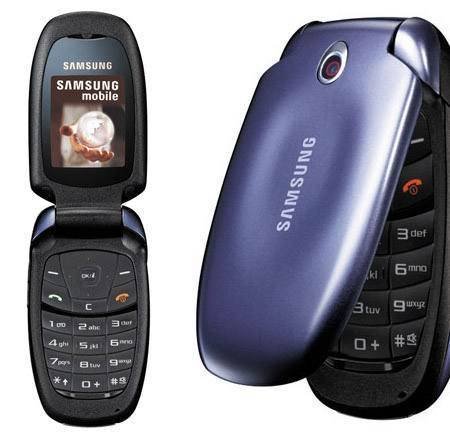
\includegraphics[trim={12mm 14mm 12mm 14mm},clip, width=\sizeP\textwidth]{fig/visual/ILSVRC2012_val_00000089.JPEG}&
	\fig[\sizeS]{visual/VGG16_GradCAM_ILSVRC2012_val_00000089.png} &
	\fig[\sizeS]{visual/VGG16_GradCAMPlusPlus_ILSVRC2012_val_00000089.png} &
	\fig[\sizeS]{visual/VGG16_ScoreCAM_ILSVRC2012_val_00000089.png} &
	\fig[\sizeS]{visual/VGG16_AblationCAM_ILSVRC2012_val_00000089.png} &
	\fig[\sizeS]{visual/VGG16_XGradCAM_ILSVRC2012_val_00000089.png} & 
	\fig[\sizeS]{visual/VGG16_OptCAM_ILSVRC2012_val_00000089.png}  \\
	Cellphone &&&&&& \\
	\fig[\sizeS]{visual/ILSVRC2012_val_00000748.png}&
	\fig[\sizeS]{visual/VGG16_GradCAM_ILSVRC2012_val_00000748.png} &
	\fig[\sizeS]{visual/VGG16_GradCAMPlusPlus_ILSVRC2012_val_00000748.png} &
	\fig[\sizeS]{visual/VGG16_ScoreCAM_ILSVRC2012_val_00000748.png} &
	\fig[\sizeS]{visual/VGG16_AblationCAM_ILSVRC2012_val_00000748.png} &
	\fig[\sizeS]{visual/VGG16_XGradCAM_ILSVRC2012_val_00000748.png} & 
	\fig[\sizeS]{visual/VGG16_OptCAM_ILSVRC2012_val_00000748.png}  \\
	Miniature Schnauzer &&&&&& \\
	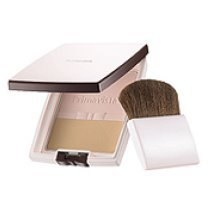
\includegraphics[trim={2mm 3mm 6mm 1mm},clip, width=\sizeP\textwidth]{fig/visual/ILSVRC2012_val_00000769.JPEG}&
	\fig[\sizeS]{visual/VGG16_GradCAM_ILSVRC2012_val_00000769.png} &
	\fig[\sizeS]{visual/VGG16_GradCAMPlusPlus_ILSVRC2012_val_00000769.png} &
	\fig[\sizeS]{visual/VGG16_ScoreCAM_ILSVRC2012_val_00000769.png} &
	\fig[\sizeS]{visual/VGG16_AblationCAM_ILSVRC2012_val_00000769.png} &
	\fig[\sizeS]{visual/VGG16_XGradCAM_ILSVRC2012_val_00000769.png} & 
	\fig[\sizeS]{visual/VGG16_OptCAM_ILSVRC2012_val_00000769.png}  \\
	Face Powder &&&&&& \\
	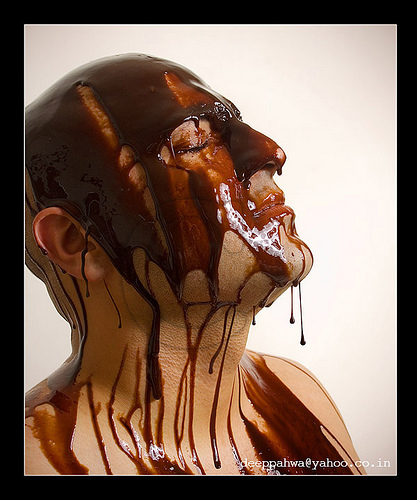
\includegraphics[trim={2mm 6mm 2mm 6mm},clip, width=\sizeP\textwidth]{fig/visual/ILSVRC2012_val_00000782.JPEG}&
	\fig[\sizeS]{visual/VGG16_GradCAM_ILSVRC2012_val_00000782.png} &
	\fig[\sizeS]{visual/VGG16_GradCAMPlusPlus_ILSVRC2012_val_00000782.png} &
	\fig[\sizeS]{visual/VGG16_ScoreCAM_ILSVRC2012_val_00000782.png} &
	\fig[\sizeS]{visual/VGG16_AblationCAM_ILSVRC2012_val_00000782.png} &
	\fig[\sizeS]{visual/VGG16_XGradCAM_ILSVRC2012_val_00000782.png} & 
	\fig[\sizeS]{visual/VGG16_OptCAM_ILSVRC2012_val_00000782.png}  \\
	Chocolate Sauce &&&&&& \\
	\fig[\sizeS]{visual/ILSVRC2012_val_00001113.png}&
	\fig[\sizeS]{visual/VGG16_GradCAM_ILSVRC2012_val_00001113.png} &
	\fig[\sizeS]{visual/VGG16_GradCAMPlusPlus_ILSVRC2012_val_00001113.png} &
	\fig[\sizeS]{visual/VGG16_ScoreCAM_ILSVRC2012_val_00001113.png} &
	\fig[\sizeS]{visual/VGG16_AblationCAM_ILSVRC2012_val_00001113.png} &
	\fig[\sizeS]{visual/VGG16_XGradCAM_ILSVRC2012_val_00001113.png} & 
	\fig[\sizeS]{visual/VGG16_OptCAM_ILSVRC2012_val_00001113.png}  \\
	Komondor &&&&&& \\
 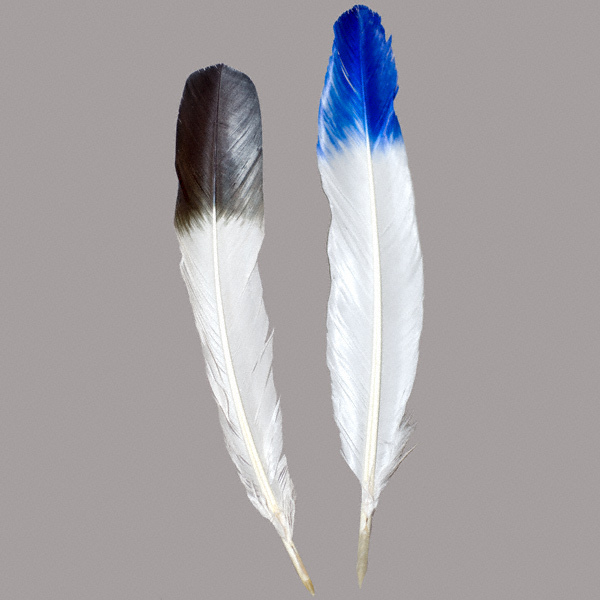
\includegraphics[trim={14mm 16mm 14mm 12mm},clip, width=\sizeP\textwidth]{fig/visual/ILSVRC2012_val_00001345.JPEG}&
	\fig[\sizeS]{visual/VGG16_GradCAM_ILSVRC2012_val_00001345.png} &
	\fig[\sizeS]{visual/VGG16_GradCAMPlusPlus_ILSVRC2012_val_00001345.png} &
	\fig[\sizeS]{visual/VGG16_ScoreCAM_ILSVRC2012_val_00001345.png} &
	\fig[\sizeS]{visual/VGG16_AblationCAM_ILSVRC2012_val_00001345.png} &
	\fig[\sizeS]{visual/VGG16_XGradCAM_ILSVRC2012_val_00001345.png} & 
	\fig[\sizeS]{visual/VGG16_OptCAM_ILSVRC2012_val_00001345.png}  \\
	Quill &&&&&& \\
 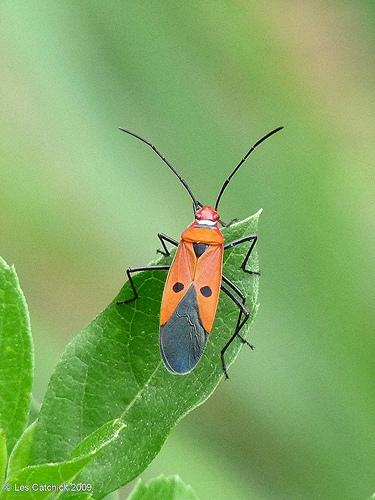
\includegraphics[trim={5mm 14mm 5mm 14mm},clip, width=\sizeP\textwidth]{fig/visual/ILSVRC2012_val_00001529.JPEG}&
	\fig[\sizeS]{visual/VGG16_GradCAM_ILSVRC2012_val_00001529.png} &
	\fig[\sizeS]{visual/VGG16_GradCAMPlusPlus_ILSVRC2012_val_00001529.png} &
	\fig[\sizeS]{visual/VGG16_ScoreCAM_ILSVRC2012_val_00001529.png} &
	\fig[\sizeS]{visual/VGG16_AblationCAM_ILSVRC2012_val_00001529.png} &
	\fig[\sizeS]{visual/VGG16_XGradCAM_ILSVRC2012_val_00001529.png} & 
	\fig[\sizeS]{visual/VGG16_OptCAM_ILSVRC2012_val_00001529.png}  \\
	Longicorn &&&&&& \\
 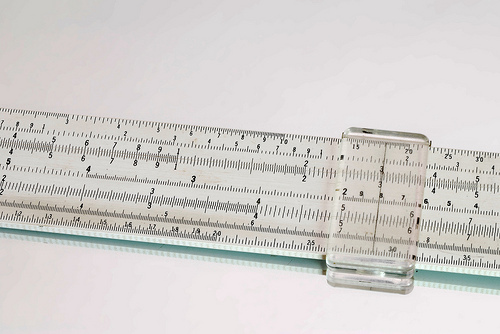
\includegraphics[trim={8mm 1mm 8mm 1mm},clip, width=\sizeP\textwidth]{fig/visual/ILSVRC2012_val_00001635.JPEG}&
	\fig[\sizeS]{visual/VGG16_GradCAM_ILSVRC2012_val_00001635.png} &
	\fig[\sizeS]{visual/VGG16_GradCAMPlusPlus_ILSVRC2012_val_00001635.png} &
	\fig[\sizeS]{visual/VGG16_ScoreCAM_ILSVRC2012_val_00001635.png} &
	\fig[\sizeS]{visual/VGG16_AblationCAM_ILSVRC2012_val_00001635.png} &
	\fig[\sizeS]{visual/VGG16_XGradCAM_ILSVRC2012_val_00001635.png} & 
	\fig[\sizeS]{visual/VGG16_OptCAM_ILSVRC2012_val_00001635.png}  \\
	Slide Rule &&&&&& \\
\end{tabular}
% \vspace{5pt}
\caption{Saliency maps obtained from ImageNet example images using different methods on VGG16.}
\label{fig:imagenet-vis-more-vgg}
\end{figure*}

% \begin{figure*}[t]
\newcommand{\sizeP}{.14}
\newcommand{\sizeS}{.14}
\newcommand{\hh}{.175\textwidth}
\newcommand{\ww}{.200\textwidth}
\scriptsize
\centering
\setlength{\tabcolsep}{3pt}
\begin{tabular}{ccccccc}
	Input image  &  Grad-CAM  & G-CAM++ & Score-CAM & Ablation-CAM & XG-CAM & Opti-CAM (ours) \\
        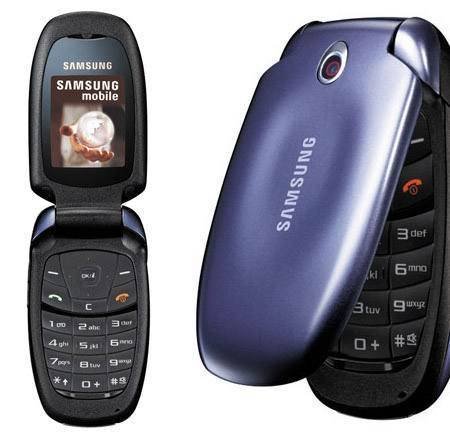
\includegraphics[trim={12mm 14mm 12mm 14mm},clip, width=\sizeP\textwidth]{fig/visual/ILSVRC2012_val_00000089.JPEG}&
	\fig[\sizeS]{visual/Resnet50_GradCAM_ILSVRC2012_val_00000089.png} &
	\fig[\sizeS]{visual/Resnet50_GradCAMPlusPlus_ILSVRC2012_val_00000089.png} &
	\fig[\sizeS]{visual/Resnet50_ScoreCAM_ILSVRC2012_val_00000089.png} &
	\fig[\sizeS]{visual/Resnet50_AblationCAM_ILSVRC2012_val_00000089.png} &
	\fig[\sizeS]{visual/Resnet50_XGradCAM_ILSVRC2012_val_00000089.png} & 
	\fig[\sizeS]{visual/Resnet50_OptCAM_ILSVRC2012_val_00000089.png}  \\
	Cellphone &&&&&& \\
	\fig[\sizeS]{visual/ILSVRC2012_val_00000748.png}&
	\fig[\sizeS]{visual/Resnet50_GradCAM_ILSVRC2012_val_00000748.png} &
	\fig[\sizeS]{visual/Resnet50_GradCAMPlusPlus_ILSVRC2012_val_00000748.png} &
	\fig[\sizeS]{visual/Resnet50_ScoreCAM_ILSVRC2012_val_00000748.png} &
	\fig[\sizeS]{visual/Resnet50_AblationCAM_ILSVRC2012_val_00000748.png} &
	\fig[\sizeS]{visual/Resnet50_XGradCAM_ILSVRC2012_val_00000748.png} & 
	\fig[\sizeS]{visual/Resnet50_OptCAM_ILSVRC2012_val_00000748.png}  \\
	Miniature Schnauzer &&&&&& \\
	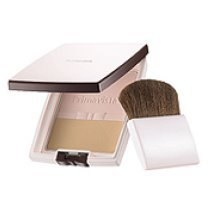
\includegraphics[trim={2mm 3mm 6mm 1mm},clip, width=\sizeP\textwidth]{fig/visual/ILSVRC2012_val_00000769.JPEG}&
	\fig[\sizeS]{visual/Resnet50_GradCAM_ILSVRC2012_val_00000769.png} &
	\fig[\sizeS]{visual/Resnet50_GradCAMPlusPlus_ILSVRC2012_val_00000769.png} &
	\fig[\sizeS]{visual/Resnet50_ScoreCAM_ILSVRC2012_val_00000769.png} &
	\fig[\sizeS]{visual/Resnet50_AblationCAM_ILSVRC2012_val_00000769.png} &
	\fig[\sizeS]{visual/Resnet50_XGradCAM_ILSVRC2012_val_00000769.png} & 
	\fig[\sizeS]{visual/Resnet50_OptCAM_ILSVRC2012_val_00000769.png}  \\
	Face Powder &&&&&& \\
	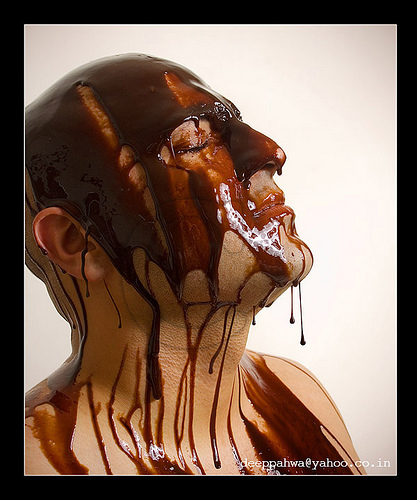
\includegraphics[trim={2mm 6mm 2mm 6mm},clip, width=\sizeP\textwidth]{fig/visual/ILSVRC2012_val_00000782.JPEG}&
	\fig[\sizeS]{visual/Resnet50_GradCAM_ILSVRC2012_val_00000782.png} &
	\fig[\sizeS]{visual/Resnet50_GradCAMPlusPlus_ILSVRC2012_val_00000782.png} &
	\fig[\sizeS]{visual/Resnet50_ScoreCAM_ILSVRC2012_val_00000782.png} &
	\fig[\sizeS]{visual/Resnet50_AblationCAM_ILSVRC2012_val_00000782.png} &
	\fig[\sizeS]{visual/Resnet50_XGradCAM_ILSVRC2012_val_00000782.png} & 
	\fig[\sizeS]{visual/Resnet50_OptCAM_ILSVRC2012_val_00000782.png}  \\
	Chocolate Sauce &&&&&& \\
	\fig[\sizeS]{visual/ILSVRC2012_val_00001113.png}&
	\fig[\sizeS]{visual/Resnet50_GradCAM_ILSVRC2012_val_00001113.png} &
	\fig[\sizeS]{visual/Resnet50_GradCAMPlusPlus_ILSVRC2012_val_00001113.png} &
	\fig[\sizeS]{visual/Resnet50_ScoreCAM_ILSVRC2012_val_00001113.png} &
	\fig[\sizeS]{visual/Resnet50_AblationCAM_ILSVRC2012_val_00001113.png} &
	\fig[\sizeS]{visual/Resnet50_XGradCAM_ILSVRC2012_val_00001113.png} & 
	\fig[\sizeS]{visual/Resnet50_OptCAM_ILSVRC2012_val_00001113.png}  \\
	Komondor &&&&&& \\
 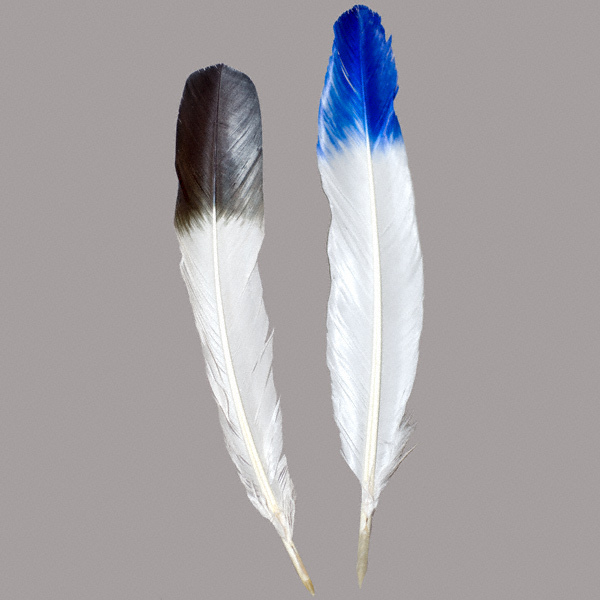
\includegraphics[trim={14mm 16mm 14mm 12mm},clip, width=\sizeP\textwidth]{fig/visual/ILSVRC2012_val_00001345.JPEG}&
	\fig[\sizeS]{visual/Resnet50_GradCAM_ILSVRC2012_val_00001345.png} &
	\fig[\sizeS]{visual/Resnet50_GradCAMPlusPlus_ILSVRC2012_val_00001345.png} &
	\fig[\sizeS]{visual/Resnet50_ScoreCAM_ILSVRC2012_val_00001345.png} &
	\fig[\sizeS]{visual/Resnet50_AblationCAM_ILSVRC2012_val_00001345.png} &
	\fig[\sizeS]{visual/Resnet50_XGradCAM_ILSVRC2012_val_00001345.png} & 
	\fig[\sizeS]{visual/Resnet50_OptCAM_ILSVRC2012_val_00001345.png}  \\
	Quill &&&&&& \\
 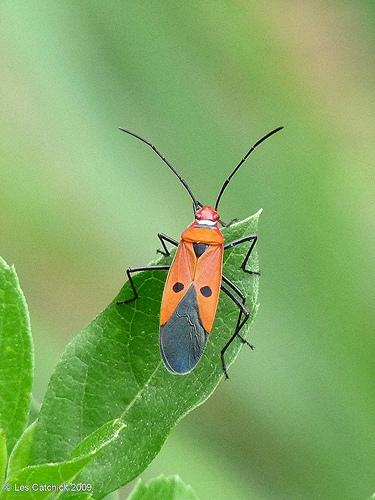
\includegraphics[trim={5mm 14mm 5mm 14mm},clip, width=\sizeP\textwidth]{fig/visual/ILSVRC2012_val_00001529.JPEG}&
	\fig[\sizeS]{visual/Resnet50_GradCAM_ILSVRC2012_val_00001529.png} &
	\fig[\sizeS]{visual/Resnet50_GradCAMPlusPlus_ILSVRC2012_val_00001529.png} &
	\fig[\sizeS]{visual/Resnet50_ScoreCAM_ILSVRC2012_val_00001529.png} &
	\fig[\sizeS]{visual/Resnet50_AblationCAM_ILSVRC2012_val_00001529.png} &
	\fig[\sizeS]{visual/Resnet50_XGradCAM_ILSVRC2012_val_00001529.png} & 
	\fig[\sizeS]{visual/Resnet50_OptCAM_ILSVRC2012_val_00001529.png}  \\
	Longicorn &&&&&& \\
 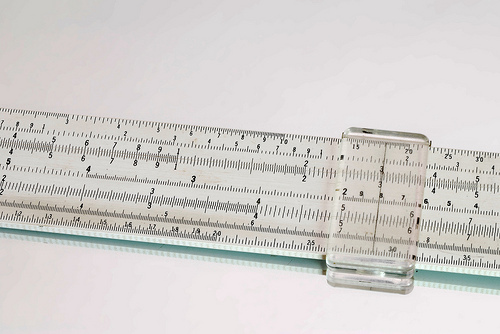
\includegraphics[trim={8mm 1mm 8mm 1mm},clip, width=\sizeP\textwidth]{fig/visual/ILSVRC2012_val_00001635.JPEG}&
	\fig[\sizeS]{visual/Resnet50_GradCAM_ILSVRC2012_val_00001635.png} &
	\fig[\sizeS]{visual/Resnet50_GradCAMPlusPlus_ILSVRC2012_val_00001635.png} &
	\fig[\sizeS]{visual/Resnet50_ScoreCAM_ILSVRC2012_val_00001635.png} &
	\fig[\sizeS]{visual/Resnet50_AblationCAM_ILSVRC2012_val_00001635.png} &
	\fig[\sizeS]{visual/Resnet50_XGradCAM_ILSVRC2012_val_00001635.png} & 
	\fig[\sizeS]{visual/Resnet50_OptCAM_ILSVRC2012_val_00001635.png}  \\
	Slide Rule &&&&&& \\
\end{tabular}
% \vspace{5pt}
\caption{Saliency maps obtained from ImageNet example images using different methods on ResNet50.}
\label{fig:imagenet-vis-more-res}
\end{figure*}

% % \begin{figure*}[t]
\newcommand{\sizeP}{.12}
\newcommand{\sizeS}{.12}
\newcommand{\hh}{.175\textwidth}
\newcommand{\ww}{.200\textwidth}
\tiny
\centering
\setlength{\tabcolsep}{1pt}
\begin{tabular}{cccccccc}
	Input image  &  Grad-CAM  & G-CAM++ & Score-CAM & XG-CAM & Raw Att. & Rollout & Opti-CAM (ours) \\
        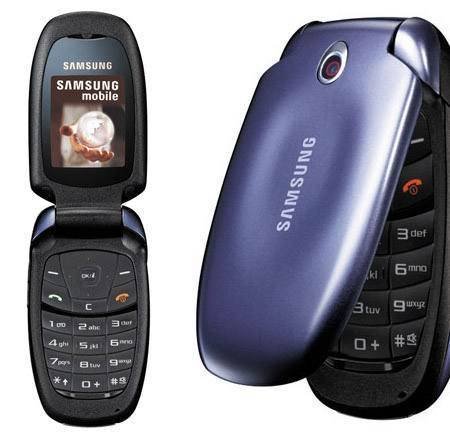
\includegraphics[trim={12mm 14mm 12mm 14mm},clip, width=\sizeP\textwidth]{fig/visual/ILSVRC2012_val_00000089.JPEG}&
	\fig[\sizeS]{visual/ViT_GradCAM_ILSVRC2012_val_00000089.png} &
	\fig[\sizeS]{visual/ViT_GradCAMPlusPlus_ILSVRC2012_val_00000089.png} &
	\fig[\sizeS]{visual/ViT_ScoreCAM_ILSVRC2012_val_00000089.png} &
	\fig[\sizeS]{visual/ViT_XGradCAM_ILSVRC2012_val_00000089.png} & 
        \fig[\sizeS]{visual/ViT_RawAttention_ILSVRC2012_val_00000089.png} &
        \fig[\sizeS]{visual/ViT_RolloutMean_ILSVRC2012_val_00000089.png} &
	\fig[\sizeS]{visual/ViT_OptiCAM_ILSVRC2012_val_00000089.png}  \\
	Cellphone &&&&&& \\
	\fig[\sizeS]{visual/ILSVRC2012_val_00000748.png}&
	\fig[\sizeS]{visual/ViT_GradCAM_ILSVRC2012_val_00000748.png} &
	\fig[\sizeS]{visual/ViT_GradCAMPlusPlus_ILSVRC2012_val_00000748.png} &
	\fig[\sizeS]{visual/ViT_ScoreCAM_ILSVRC2012_val_00000748.png} &
	\fig[\sizeS]{visual/ViT_XGradCAM_ILSVRC2012_val_00000748.png} & 
        \fig[\sizeS]{visual/ViT_RawAttention_ILSVRC2012_val_00000748.png} &
        \fig[\sizeS]{visual/ViT_RolloutMean_ILSVRC2012_val_00000748.png} &
	\fig[\sizeS]{visual/ViT_OptiCAM_ILSVRC2012_val_00000748.png}  \\
	Miniature Schnauzer &&&&&& \\
	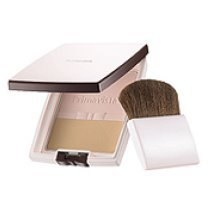
\includegraphics[trim={2mm 3mm 6mm 1mm},clip, width=\sizeP\textwidth]{fig/visual/ILSVRC2012_val_00000769.JPEG}&
	\fig[\sizeS]{visual/ViT_GradCAM_ILSVRC2012_val_00000769.png} &
	\fig[\sizeS]{visual/ViT_GradCAMPlusPlus_ILSVRC2012_val_00000769.png} &
	\fig[\sizeS]{visual/ViT_ScoreCAM_ILSVRC2012_val_00000769.png} &
	\fig[\sizeS]{visual/ViT_XGradCAM_ILSVRC2012_val_00000769.png} & 
        \fig[\sizeS]{visual/ViT_RawAttention_ILSVRC2012_val_00000769.png} &
        \fig[\sizeS]{visual/ViT_RolloutMean_ILSVRC2012_val_00000769.png} &
	\fig[\sizeS]{visual/ViT_OptiCAM_ILSVRC2012_val_00000769.png}  \\
	Face Powder &&&&&& \\
	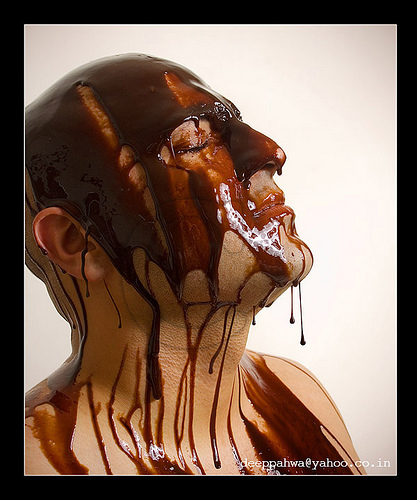
\includegraphics[trim={2mm 6mm 2mm 6mm},clip, width=\sizeP\textwidth]{fig/visual/ILSVRC2012_val_00000782.JPEG}&
	\fig[\sizeS]{visual/ViT_GradCAM_ILSVRC2012_val_00000782.png} &
	\fig[\sizeS]{visual/ViT_GradCAMPlusPlus_ILSVRC2012_val_00000782.png} &
	\fig[\sizeS]{visual/ViT_ScoreCAM_ILSVRC2012_val_00000782.png} &
	\fig[\sizeS]{visual/ViT_XGradCAM_ILSVRC2012_val_00000782.png} & 
        \fig[\sizeS]{visual/ViT_RawAttention_ILSVRC2012_val_00000782.png} &
        \fig[\sizeS]{visual/ViT_RolloutMean_ILSVRC2012_val_00000782.png} &
	\fig[\sizeS]{visual/ViT_OptiCAM_ILSVRC2012_val_00000782.png}  \\
	Chocolate Sauce &&&&&& \\
	\fig[\sizeS]{visual/ILSVRC2012_val_00001113.png}&
	\fig[\sizeS]{visual/ViT_GradCAM_ILSVRC2012_val_00001113.png} &
	\fig[\sizeS]{visual/ViT_GradCAMPlusPlus_ILSVRC2012_val_00001113.png} &
	\fig[\sizeS]{visual/ViT_ScoreCAM_ILSVRC2012_val_00001113.png} &
	\fig[\sizeS]{visual/ViT_XGradCAM_ILSVRC2012_val_00001113.png} & 
        \fig[\sizeS]{visual/ViT_RawAttention_ILSVRC2012_val_00001113.png} &
        \fig[\sizeS]{visual/ViT_RolloutMean_ILSVRC2012_val_00001113.png} &
	\fig[\sizeS]{visual/ViT_OptiCAM_ILSVRC2012_val_00001113.png}  \\
	Komondor &&&&&& \\
 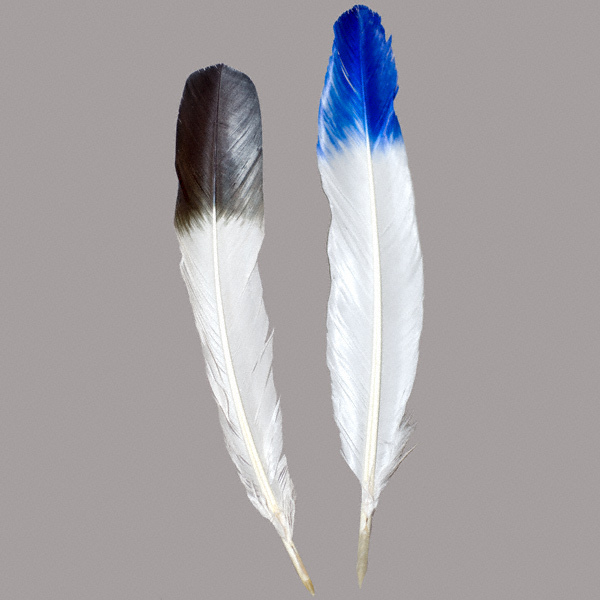
\includegraphics[trim={14mm 16mm 14mm 12mm},clip, width=\sizeP\textwidth]{fig/visual/ILSVRC2012_val_00001345.JPEG}&
	\fig[\sizeS]{visual/ViT_GradCAM_ILSVRC2012_val_00001345.png} &
	\fig[\sizeS]{visual/ViT_GradCAMPlusPlus_ILSVRC2012_val_00001345.png} &
	\fig[\sizeS]{visual/ViT_ScoreCAM_ILSVRC2012_val_00001345.png} &
	\fig[\sizeS]{visual/ViT_XGradCAM_ILSVRC2012_val_00001345.png} & 
        \fig[\sizeS]{visual/ViT_RawAttention_ILSVRC2012_val_00001345.png} &
        \fig[\sizeS]{visual/ViT_RolloutMean_ILSVRC2012_val_00001345.png} &
	\fig[\sizeS]{visual/ViT_OptiCAM_ILSVRC2012_val_00001345.png}  \\
	Quill &&&&&& \\
 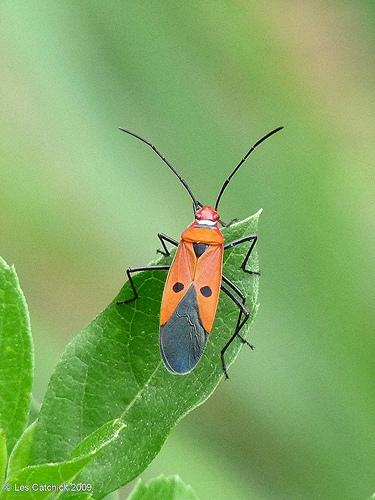
\includegraphics[trim={5mm 14mm 5mm 14mm},clip, width=\sizeP\textwidth]{fig/visual/ILSVRC2012_val_00001529.JPEG}&
	\fig[\sizeS]{visual/ViT_GradCAM_ILSVRC2012_val_00001529.png} &
	\fig[\sizeS]{visual/ViT_GradCAMPlusPlus_ILSVRC2012_val_00001529.png} &
	\fig[\sizeS]{visual/ViT_ScoreCAM_ILSVRC2012_val_00001529.png} &
	\fig[\sizeS]{visual/ViT_XGradCAM_ILSVRC2012_val_00001529.png} & 
        \fig[\sizeS]{visual/ViT_RawAttention_ILSVRC2012_val_00001529.png} &
        \fig[\sizeS]{visual/ViT_RolloutMean_ILSVRC2012_val_00001529.png} &
	\fig[\sizeS]{visual/ViT_OptiCAM_ILSVRC2012_val_00001529.png}  \\
	Longicorn &&&&&& \\
 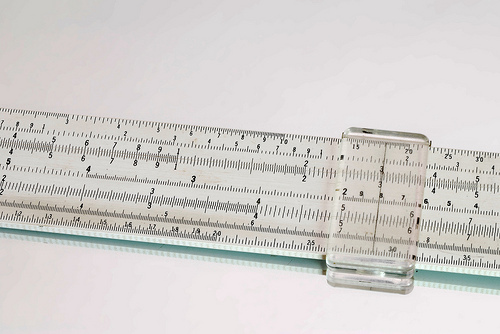
\includegraphics[trim={8mm 1mm 8mm 1mm},clip, width=\sizeP\textwidth]{fig/visual/ILSVRC2012_val_00001635.JPEG}&
	\fig[\sizeS]{visual/ViT_GradCAM_ILSVRC2012_val_00001635.png} &
	\fig[\sizeS]{visual/ViT_GradCAMPlusPlus_ILSVRC2012_val_00001635.png} &
	\fig[\sizeS]{visual/ViT_ScoreCAM_ILSVRC2012_val_00001635.png} &
	\fig[\sizeS]{visual/ViT_XGradCAM_ILSVRC2012_val_00001635.png} & 
        \fig[\sizeS]{visual/ViT_RawAttention_ILSVRC2012_val_00001635.png} &
        \fig[\sizeS]{visual/ViT_RolloutMean_ILSVRC2012_val_00001635.png} &
	\fig[\sizeS]{visual/ViT_OptiCAM_ILSVRC2012_val_00001635.png}  \\
	Slide Rule &&&&&& \\
\end{tabular}
% \vspace{5pt}
\caption{Saliency maps obtained from ImageNet example images using different methods on ViT.}
\label{fig:imagenet-vis-more-vit}
\end{figure*}

% % \begin{figure*}[t]
\newcommand{\sizeP}{.12}
\newcommand{\sizeS}{.12}
\newcommand{\hh}{.175\textwidth}
\newcommand{\ww}{.200\textwidth}
\tiny
\centering
\setlength{\tabcolsep}{1pt}
\begin{tabular}{cccccccc}
	Input image  &  Grad-CAM  & G-CAM++ & Score-CAM & XG-CAM & Raw Att. & Rollout & Opti-CAM (ours) \\
        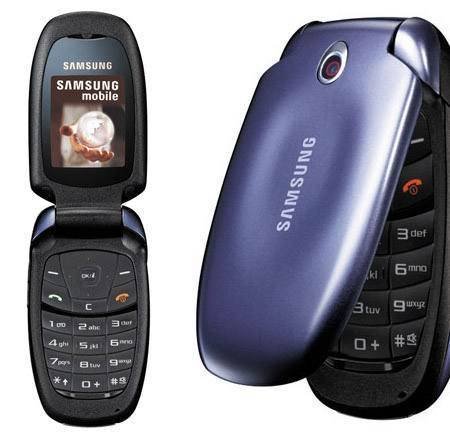
\includegraphics[trim={12mm 14mm 12mm 14mm},clip, width=\sizeP\textwidth]{fig/visual/ILSVRC2012_val_00000089.JPEG}&
	\fig[\sizeS]{visual/DeitBase_GradCAM_ILSVRC2012_val_00000089.png} &
	\fig[\sizeS]{visual/DeitBase_GradCAMPlusPlus_ILSVRC2012_val_00000089.png} &
	\fig[\sizeS]{visual/DeitBase_ScoreCAM_ILSVRC2012_val_00000089.png} &
	\fig[\sizeS]{visual/DeitBase_XGradCAM_ILSVRC2012_val_00000089.png} & 
        \fig[\sizeS]{visual/DeitBase_RawAttention_ILSVRC2012_val_00000089.png} &
        \fig[\sizeS]{visual/DeitBase_RolloutMean_ILSVRC2012_val_00000089.png} &
	\fig[\sizeS]{visual/DeitBase_OptiCAM_ILSVRC2012_val_00000089.png}  \\
	Cellphone &&&&&& \\
	\fig[\sizeS]{visual/ILSVRC2012_val_00000748.png}&
	\fig[\sizeS]{visual/DeitBase_GradCAM_ILSVRC2012_val_00000748.png} &
	\fig[\sizeS]{visual/DeitBase_GradCAMPlusPlus_ILSVRC2012_val_00000748.png} &
	\fig[\sizeS]{visual/DeitBase_ScoreCAM_ILSVRC2012_val_00000748.png} &
	\fig[\sizeS]{visual/DeitBase_XGradCAM_ILSVRC2012_val_00000748.png} & 
        \fig[\sizeS]{visual/DeitBase_RawAttention_ILSVRC2012_val_00000748.png} &
        \fig[\sizeS]{visual/DeitBase_RolloutMean_ILSVRC2012_val_00000748.png} &
	\fig[\sizeS]{visual/DeitBase_OptiCAM_ILSVRC2012_val_00000748.png}  \\
	Miniature Schnauzer &&&&&& \\
	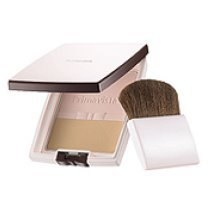
\includegraphics[trim={2mm 3mm 6mm 1mm},clip, width=\sizeP\textwidth]{fig/visual/ILSVRC2012_val_00000769.JPEG}&
	\fig[\sizeS]{visual/DeitBase_GradCAM_ILSVRC2012_val_00000769.png} &
	\fig[\sizeS]{visual/DeitBase_GradCAMPlusPlus_ILSVRC2012_val_00000769.png} &
	\fig[\sizeS]{visual/DeitBase_ScoreCAM_ILSVRC2012_val_00000769.png} &
	\fig[\sizeS]{visual/DeitBase_XGradCAM_ILSVRC2012_val_00000769.png} & 
        \fig[\sizeS]{visual/DeitBase_RawAttention_ILSVRC2012_val_00000769.png} &
        \fig[\sizeS]{visual/DeitBase_RolloutMean_ILSVRC2012_val_00000769.png} &
	\fig[\sizeS]{visual/DeitBase_OptiCAM_ILSVRC2012_val_00000769.png}  \\
	Face Powder &&&&&& \\
	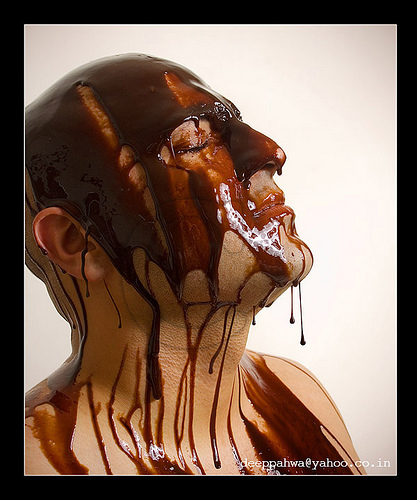
\includegraphics[trim={2mm 6mm 2mm 6mm},clip, width=\sizeP\textwidth]{fig/visual/ILSVRC2012_val_00000782.JPEG}&
	\fig[\sizeS]{visual/DeitBase_GradCAM_ILSVRC2012_val_00000782.png} &
	\fig[\sizeS]{visual/DeitBase_GradCAMPlusPlus_ILSVRC2012_val_00000782.png} &
	\fig[\sizeS]{visual/DeitBase_ScoreCAM_ILSVRC2012_val_00000782.png} &
	\fig[\sizeS]{visual/DeitBase_XGradCAM_ILSVRC2012_val_00000782.png} & 
        \fig[\sizeS]{visual/DeitBase_RawAttention_ILSVRC2012_val_00000782.png} &
        \fig[\sizeS]{visual/DeitBase_RolloutMean_ILSVRC2012_val_00000782.png} &
	\fig[\sizeS]{visual/DeitBase_OptiCAM_ILSVRC2012_val_00000782.png}  \\
	Chocolate Sauce &&&&&& \\
	\fig[\sizeS]{visual/ILSVRC2012_val_00001113.png}&
	\fig[\sizeS]{visual/DeitBase_GradCAM_ILSVRC2012_val_00001113.png} &
	\fig[\sizeS]{visual/DeitBase_GradCAMPlusPlus_ILSVRC2012_val_00001113.png} &
	\fig[\sizeS]{visual/DeitBase_ScoreCAM_ILSVRC2012_val_00001113.png} &
	\fig[\sizeS]{visual/DeitBase_XGradCAM_ILSVRC2012_val_00001113.png} & 
        \fig[\sizeS]{visual/DeitBase_RawAttention_ILSVRC2012_val_00001113.png} &
        \fig[\sizeS]{visual/DeitBase_RolloutMean_ILSVRC2012_val_00001113.png} &
	\fig[\sizeS]{visual/DeitBase_OptiCAM_ILSVRC2012_val_00001113.png}  \\
	Komondor &&&&&& \\
 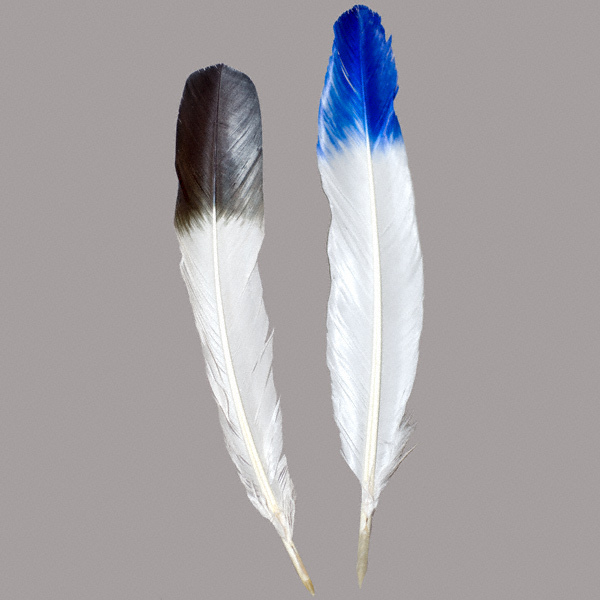
\includegraphics[trim={14mm 16mm 14mm 12mm},clip, width=\sizeP\textwidth]{fig/visual/ILSVRC2012_val_00001345.JPEG}&
	\fig[\sizeS]{visual/DeitBase_GradCAM_ILSVRC2012_val_00001345.png} &
	\fig[\sizeS]{visual/DeitBase_GradCAMPlusPlus_ILSVRC2012_val_00001345.png} &
	\fig[\sizeS]{visual/DeitBase_ScoreCAM_ILSVRC2012_val_00001345.png} &
	\fig[\sizeS]{visual/DeitBase_XGradCAM_ILSVRC2012_val_00001345.png} & 
        \fig[\sizeS]{visual/DeitBase_RawAttention_ILSVRC2012_val_00001345.png} &
        \fig[\sizeS]{visual/DeitBase_RolloutMean_ILSVRC2012_val_00001345.png} &
	\fig[\sizeS]{visual/DeitBase_OptiCAM_ILSVRC2012_val_00001345.png}  \\
	Quill &&&&&& \\
 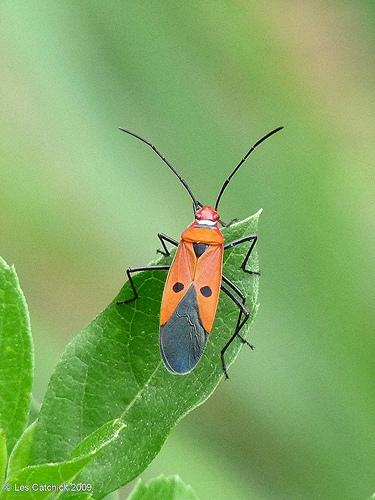
\includegraphics[trim={5mm 14mm 5mm 14mm},clip, width=\sizeP\textwidth]{fig/visual/ILSVRC2012_val_00001529.JPEG}&
	\fig[\sizeS]{visual/DeitBase_GradCAM_ILSVRC2012_val_00001529.png} &
	\fig[\sizeS]{visual/DeitBase_GradCAMPlusPlus_ILSVRC2012_val_00001529.png} &
	\fig[\sizeS]{visual/DeitBase_ScoreCAM_ILSVRC2012_val_00001529.png} &
	\fig[\sizeS]{visual/DeitBase_XGradCAM_ILSVRC2012_val_00001529.png} & 
        \fig[\sizeS]{visual/DeitBase_RawAttention_ILSVRC2012_val_00001529.png} &
        \fig[\sizeS]{visual/DeitBase_RolloutMean_ILSVRC2012_val_00001529.png} &
	\fig[\sizeS]{visual/DeitBase_OptiCAM_ILSVRC2012_val_00001529.png}  \\
	Longicorn &&&&&& \\
 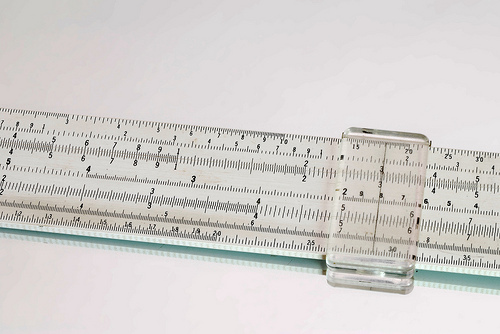
\includegraphics[trim={8mm 1mm 8mm 1mm},clip, width=\sizeP\textwidth]{fig/visual/ILSVRC2012_val_00001635.JPEG}&
	\fig[\sizeS]{visual/DeitBase_GradCAM_ILSVRC2012_val_00001635.png} &
	\fig[\sizeS]{visual/DeitBase_GradCAMPlusPlus_ILSVRC2012_val_00001635.png} &
	\fig[\sizeS]{visual/DeitBase_ScoreCAM_ILSVRC2012_val_00001635.png} &
	\fig[\sizeS]{visual/DeitBase_XGradCAM_ILSVRC2012_val_00001635.png} & 
        \fig[\sizeS]{visual/DeitBase_RawAttention_ILSVRC2012_val_00001635.png} &
        \fig[\sizeS]{visual/DeitBase_RolloutMean_ILSVRC2012_val_00001635.png} &
	\fig[\sizeS]{visual/DeitBase_OptiCAM_ILSVRC2012_val_00001635.png}  \\
	Slide Rule &&&&&& \\
\end{tabular}
\vspace{5pt}
\caption{Saliency maps obtained from ImageNet example images using different methods on DeiT.}
\label{fig:imagenet-vis-more-DeiT}
\end{figure*}

% % \begin{figure*}[t]
\newcommand{\sizeP}{.12}
\newcommand{\sizeS}{.12}
\newcommand{\hh}{.175\textwidth}
\newcommand{\ww}{.200\textwidth}
\tiny
\centering
\setlength{\tabcolsep}{1pt}
\begin{tabular}{cccccccc}
	Input image  &  Grad-CAM  & G-CAM++ & Score-CAM & XG-CAM & Raw Att. & Rollout & Opti-CAM (ours) \\
        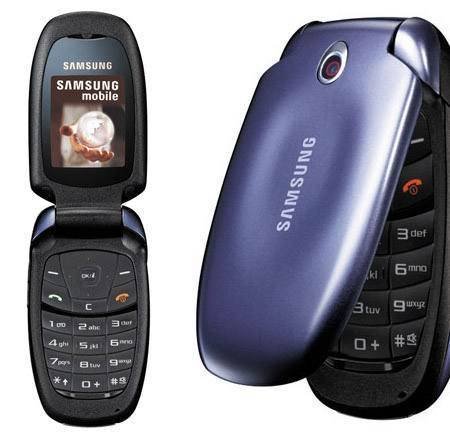
\includegraphics[trim={12mm 14mm 12mm 14mm},clip, width=\sizeP\textwidth]{fig/visual/ILSVRC2012_val_00000089.JPEG}&
	\fig[\sizeS]{visual/DeitTiny_GradCAM_ILSVRC2012_val_00000089.png} &
	\fig[\sizeS]{visual/DeitTiny_GradCAMPlusPlus_ILSVRC2012_val_00000089.png} &
	\fig[\sizeS]{visual/DeitTiny_ScoreCAM_ILSVRC2012_val_00000089.png} &
	\fig[\sizeS]{visual/DeitTiny_XGradCAM_ILSVRC2012_val_00000089.png} & 
        \fig[\sizeS]{visual/DeitTiny_RawAttention_ILSVRC2012_val_00000089.png} &
        \fig[\sizeS]{visual/DeitTiny_RolloutMean_ILSVRC2012_val_00000089.png} &
	\fig[\sizeS]{visual/DeitTiny_OptiCAM_ILSVRC2012_val_00000089.png}  \\
	Cellphone &&&&&& \\
	\fig[\sizeS]{visual/ILSVRC2012_val_00000748.png}&
	\fig[\sizeS]{visual/DeitTiny_GradCAM_ILSVRC2012_val_00000748.png} &
	\fig[\sizeS]{visual/DeitTiny_GradCAMPlusPlus_ILSVRC2012_val_00000748.png} &
	\fig[\sizeS]{visual/DeitTiny_ScoreCAM_ILSVRC2012_val_00000748.png} &
	\fig[\sizeS]{visual/DeitTiny_XGradCAM_ILSVRC2012_val_00000748.png} & 
        \fig[\sizeS]{visual/DeitTiny_RawAttention_ILSVRC2012_val_00000748.png} &
        \fig[\sizeS]{visual/DeitTiny_RolloutMean_ILSVRC2012_val_00000748.png} &
	\fig[\sizeS]{visual/DeitTiny_OptiCAM_ILSVRC2012_val_00000748.png}  \\
	Miniature Schnauzer &&&&&& \\
	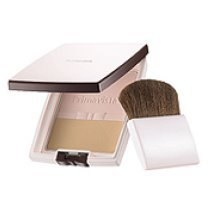
\includegraphics[trim={2mm 3mm 6mm 1mm},clip, width=\sizeP\textwidth]{fig/visual/ILSVRC2012_val_00000769.JPEG}&
	\fig[\sizeS]{visual/DeitTiny_GradCAM_ILSVRC2012_val_00000769.png} &
	\fig[\sizeS]{visual/DeitTiny_GradCAMPlusPlus_ILSVRC2012_val_00000769.png} &
	\fig[\sizeS]{visual/DeitTiny_ScoreCAM_ILSVRC2012_val_00000769.png} &
	\fig[\sizeS]{visual/DeitTiny_XGradCAM_ILSVRC2012_val_00000769.png} & 
        \fig[\sizeS]{visual/DeitTiny_RawAttention_ILSVRC2012_val_00000769.png} &
        \fig[\sizeS]{visual/DeitTiny_RolloutMean_ILSVRC2012_val_00000769.png} &
	\fig[\sizeS]{visual/DeitTiny_OptiCAM_ILSVRC2012_val_00000769.png}  \\
	Face Powder &&&&&& \\
	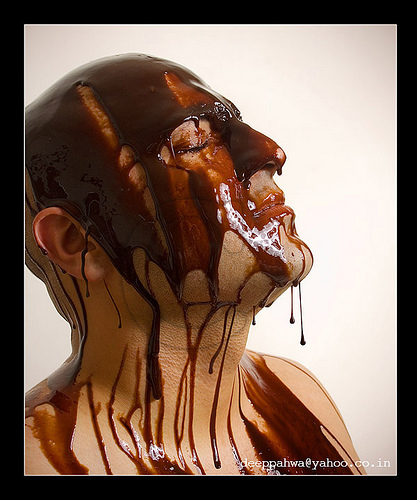
\includegraphics[trim={2mm 6mm 2mm 6mm},clip, width=\sizeP\textwidth]{fig/visual/ILSVRC2012_val_00000782.JPEG}&
	\fig[\sizeS]{visual/DeitTiny_GradCAM_ILSVRC2012_val_00000782.png} &
	\fig[\sizeS]{visual/DeitTiny_GradCAMPlusPlus_ILSVRC2012_val_00000782.png} &
	\fig[\sizeS]{visual/DeitTiny_ScoreCAM_ILSVRC2012_val_00000782.png} &
	\fig[\sizeS]{visual/DeitTiny_XGradCAM_ILSVRC2012_val_00000782.png} & 
        \fig[\sizeS]{visual/DeitTiny_RawAttention_ILSVRC2012_val_00000782.png} &
        \fig[\sizeS]{visual/DeitTiny_RolloutMean_ILSVRC2012_val_00000782.png} &
	\fig[\sizeS]{visual/DeitTiny_OptiCAM_ILSVRC2012_val_00000782.png}  \\
	Chocolate Sauce &&&&&& \\
	\fig[\sizeS]{visual/ILSVRC2012_val_00001113.png}&
	\fig[\sizeS]{visual/DeitTiny_GradCAM_ILSVRC2012_val_00001113.png} &
	\fig[\sizeS]{visual/DeitTiny_GradCAMPlusPlus_ILSVRC2012_val_00001113.png} &
	\fig[\sizeS]{visual/DeitTiny_ScoreCAM_ILSVRC2012_val_00001113.png} &
	\fig[\sizeS]{visual/DeitTiny_XGradCAM_ILSVRC2012_val_00001113.png} & 
        \fig[\sizeS]{visual/DeitTiny_RawAttention_ILSVRC2012_val_00001113.png} &
        \fig[\sizeS]{visual/DeitTiny_RolloutMean_ILSVRC2012_val_00001113.png} &
	\fig[\sizeS]{visual/DeitTiny_OptiCAM_ILSVRC2012_val_00001113.png}  \\
	Komondor &&&&&& \\
 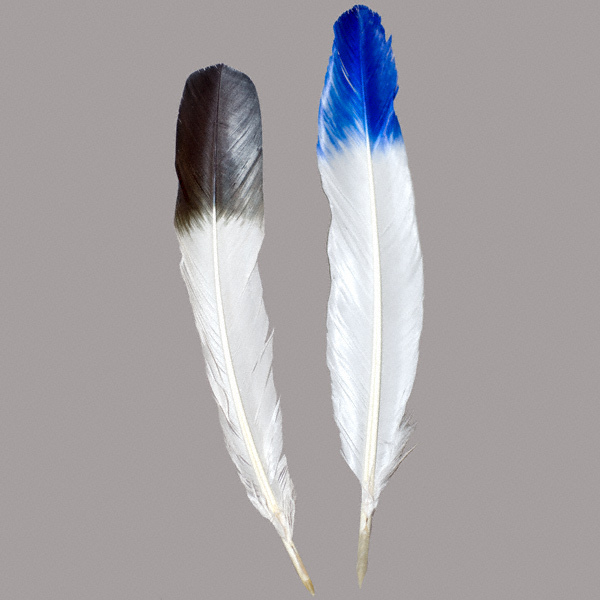
\includegraphics[trim={14mm 16mm 14mm 12mm},clip, width=\sizeP\textwidth]{fig/visual/ILSVRC2012_val_00001345.JPEG}&
	\fig[\sizeS]{visual/DeitTiny_GradCAM_ILSVRC2012_val_00001345.png} &
	\fig[\sizeS]{visual/DeitTiny_GradCAMPlusPlus_ILSVRC2012_val_00001345.png} &
	\fig[\sizeS]{visual/DeitTiny_ScoreCAM_ILSVRC2012_val_00001345.png} &
	\fig[\sizeS]{visual/DeitTiny_XGradCAM_ILSVRC2012_val_00001345.png} & 
        \fig[\sizeS]{visual/DeitTiny_RawAttention_ILSVRC2012_val_00001345.png} &
        \fig[\sizeS]{visual/DeitTiny_RolloutMean_ILSVRC2012_val_00001345.png} &
	\fig[\sizeS]{visual/DeitTiny_OptiCAM_ILSVRC2012_val_00001345.png}  \\
	Quill &&&&&& \\
 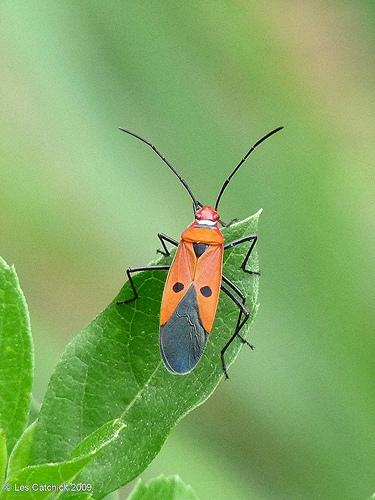
\includegraphics[trim={5mm 14mm 5mm 14mm},clip, width=\sizeP\textwidth]{fig/visual/ILSVRC2012_val_00001529.JPEG}&
	\fig[\sizeS]{visual/DeitTiny_GradCAM_ILSVRC2012_val_00001529.png} &
	\fig[\sizeS]{visual/DeitTiny_GradCAMPlusPlus_ILSVRC2012_val_00001529.png} &
	\fig[\sizeS]{visual/DeitTiny_ScoreCAM_ILSVRC2012_val_00001529.png} &
	\fig[\sizeS]{visual/DeitTiny_XGradCAM_ILSVRC2012_val_00001529.png} & 
        \fig[\sizeS]{visual/DeitTiny_RawAttention_ILSVRC2012_val_00001529.png} &
        \fig[\sizeS]{visual/DeitTiny_RolloutMean_ILSVRC2012_val_00001529.png} &
	\fig[\sizeS]{visual/DeitTiny_OptiCAM_ILSVRC2012_val_00001529.png}  \\
	Longicorn &&&&&& \\
 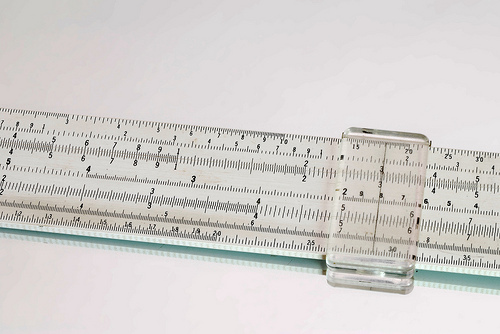
\includegraphics[trim={8mm 1mm 8mm 1mm},clip, width=\sizeP\textwidth]{fig/visual/ILSVRC2012_val_00001635.JPEG}&
	\fig[\sizeS]{visual/DeitTiny_GradCAM_ILSVRC2012_val_00001635.png} &
	\fig[\sizeS]{visual/DeitTiny_GradCAMPlusPlus_ILSVRC2012_val_00001635.png} &
	\fig[\sizeS]{visual/DeitTiny_ScoreCAM_ILSVRC2012_val_00001635.png} &
	\fig[\sizeS]{visual/DeitTiny_XGradCAM_ILSVRC2012_val_00001635.png} & 
        \fig[\sizeS]{visual/DeitTiny_RawAttention_ILSVRC2012_val_00001635.png} &
        \fig[\sizeS]{visual/DeitTiny_RolloutMean_ILSVRC2012_val_00001635.png} &
	\fig[\sizeS]{visual/DeitTiny_OptiCAM_ILSVRC2012_val_00001635.png}  \\
	Slide Rule &&&&&& \\
\end{tabular}
\vspace{5pt}
\caption{Saliency maps obtained from ImageNet example images using different methods on DeitTiny.}
\label{fig:imagenet-vis-more-DeitTiny}
\end{figure*}

% %------------------------------------------------------------------------------

% \section{More visualizations}
% \label{sec:more-vis}

% \autoref{fig:vis-chest-resnet} and \autoref{fig:vis-kvasir-resnet} present additional visualizations on Chest X-ray and Kvasir datasets using VGG16 and ResNet50. 
% Then \autoref{fig:imagenet-vis-more-vgg} and \autoref{fig:imagenet-vis-more-res}
% % \autoref{fig:imagenet-vis-more-vit} 
% show more results on ImageNet using VGG16 and ResNet50, respectively.

% Overall, we still observe that Opti-CAM captures more of the object area compared with other saliency methods and sometimes background context as well \autoref{fig:imagenet-vis-more-res}.

